\documentclass[10pt,dvips]{report}

% $Header$
% Copyright (C) 1996-2015 Pierangelo Masarati <masarati@aero.polimi.it>
% Dipartimento di Ingegneria Aerospaziale, Politecnico di Milano
%
% Parentesi: tonde, quadre, curly, dritte, doppie e angolari.
\newcommand{\plbr}[1]{ \left( #1 \right) }
\newcommand{\sqbr}[1]{ \left[ #1 \right] }
\newcommand{\cubr}[1]{ \left\{ #1 \right\} }
\newcommand{\shbr}[1]{ \left| #1 \right| }
\newcommand{\nrbr}[1]{ \left\| #1 \right\| }
\newcommand{\anbr}[1]{ \langle #1 \rangle }

% Parentesi solo a sinistra: tonde, quadre, curly, dritte, doppie e angolari.
\newcommand{\lplbr}[1]{ \left( #1 \right. }
\newcommand{\lsqbr}[1]{ \left[ #1 \right. }
\newcommand{\lcubr}[1]{ \left\{ #1 \right. }
\newcommand{\lshbr}[1]{ \left| #1 \right. }
\newcommand{\lnrbr}[1]{ \left\| #1 \right. }
\newcommand{\lanbr}[1]{ \langle #1 \right. }

% Parentesi solo a destra: tonde, quadre, curly, dritte,doppie e angolari.
\newcommand{\rplbr}[1]{ \left. #1 \right) }
\newcommand{\rsqbr}[1]{ \left. #1 \right] }
\newcommand{\rcubr}[1]{ \left. #1 \right\} }
\newcommand{\rshbr}[1]{ \left. #1 \right| }
\newcommand{\rnrbr}[1]{ \left. #1 \right\| }
\newcommand{\ranbr}[1]{ \left. #1 \rangle }

% Vettori verticali:
\newcommand{\vvect}[2]{ \begin{array}{ #1 } #2 \end{array} }
\newcommand{\cvvect}[1]{ \begin{array}{c} #1 \end{array} }
\newcommand{\lvvect}[1]{ \begin{array}{l} #1 \end{array} }
\newcommand{\rvvect}[1]{ \begin{array}{r} #1 \end{array} }

% Vettori orizzontali:
\newcommand{\hvect}[2]{ \begin{array}{ #1 } #2 \end{array} }

% Matrici:
\newcommand{\matr}[2]{ \begin{array}{ #1 } #2 \end{array} }

% Integrali: uso \intg{inf}{sup}{arg}{dvar}
\newcommand{\intg}[4]{ \int_{#1}^{#2} {#3} \ {#4} }

% Limite: uso \limt{var}{lim}{arg}
\newcommand{\limt}[3]{ \lim_{{#1} \rightarrow {#2}} {#3}}

% LogLike functions
\newcommand{\llk}[1]{\ensuremath{\mathrm{#1}}}

\newcommand{\diag}[0]{\llk{diag}}
\newcommand{\tr}[0]{\llk{tr}}
\newcommand{\sym}[0]{\llk{sym}}
\newcommand{\skw}[0]{\llk{skw}}

\newcommand{\step}[0]{\llk{step}}
\newcommand{\imp}[0]{\llk{imp}}

\newcommand{\grad}[0]{\llk{grad}}
\newcommand{\divr}[0]{\llk{div}}
\newcommand{\rot}[0]{\llk{rot}}

% In italiano ...
\newcommand{\sca}[0]{\llk{sca}}

% first, second, etc
\newcommand{\first}[0]{1\ensuremath{^{\mathrm{st}}}}    % 1^st
\newcommand{\second}[0]{2\ensuremath{^{\mathrm{nd}}}}   % 2^nd
\newcommand{\third}[0]{3\ensuremath{^{\mathrm{rd}}}}    % 3^rd
\newcommand{\rth}[0]{\ensuremath{^{\mathrm{th}}}}       %  ^th

\newcommand{\degr}[0]{\ensuremath{^{\mathrm{o}}}}

% esponenziale
\providecommand{\e}[1]{\llk{e}^{#1}}

\usepackage{graphicx}
\usepackage{amsmath}

\begin{document}

\title{\bf MBDyn Input File Format}
\author{Pierangelo Masarati \vspace{5mm}\\
    \sc Dipartimento di Ingegneria Aerospaziale \\
    \sc Politecnico di Milano
}
\date{}

\maketitle


\tableofcontents
\newpage

\chapter{Introduction}
This paper describes the format of the input data for MBDyn: 
Multi-body Analysis program.
It should be considered a syntax more than a format, since the rules of the
input allow a lot of freedom in the file format. \\
{\em
    Note: throughout the manual, a Backus-Naur-like sintax description is
    used. 
    Extensions are made, such as to put extra arguments in square brackets
    {\tt []}, mutually exclusive arguments in curl brackets {\tt \{\}},
    separated by the logical ``or'' {\tt |} operator.
    Non-terminal symbols are enclosed in angle brackets {\tt <>}, while
    terminal symbols are written in normal types.
    The association of a non-terminal with terminal or non-terminal
    symbols is performed by means of the operator `{\tt ::=}'. 
    % Special characters are enclosed in simple quotes {\tt `}, and {\tt '}.
    When required, the type of a non-terminal symbol is enforced in a ``C''
    programming language casting style, by prepending a (usually
    self-explanatory) type enclosed in plain brackets {\tt ()}.
}







\chapter{General}
The input is divided in blocks. 
This is a consequence of the fact that almost every module of the code 
needs data and each module is responsible for its data input. 
So it is natural to make each module read and interpret its data starting 
from the input phase.
Every command (or card) has the following ``grammar'':
\begin{verbatim}
    <card> ::= <description> [ : <arglist> ] ;
\end{verbatim}
{\tt arglist} is a (optional) list of arguments, that is driven by the 
{\tt description} that identifies the card. 
The keyword can be made of multiple words separated by spaces or tabs; 
the extra spaces are skipped\footnote{
    Anything that makes the ``C'' function {\tt isspace()} return {\tt true}
}, and the match is case insensitive. 
The arguments are usually separated by commas\footnote{
    A few exceptions require a colon to separate blocks of arguments;
    wherever it is feasible, those exceptions will be eliminated in future
    versions. Those cards will be marked as deprecated.
}.
A semicolon ends the card. 
Many cards allow for extra arguments that assume default values 
if not supplied by the user. 
Usually these arguments are at the end of the card and must follow some 
rules. 
A check for the existence of extra args is made, and they are read in a 
fixed sequence.
When structured arguments like matrices, vectors, or drive callers are
expected, they are parsed by dedicated functions.
Anyway, the structured data always follows the rules of the general data. 
Few exceptions are present, and will be eliminated soon.
Every data module is surrounded by the control statements {\tt begin} and
{\tt end}:
\begin{verbatim}
    begin: <module_name> ;
        ...
    end: <module_name> ;
\end{verbatim}
The general rules follow.



\section{Output}
The program outputs data to a set of files for each simulation.
The contents of the file is related to the extension of the input file.
If no input file is explicitly supplied, and input is obtained from 
{\tt stdin}, the output file name defaults to ``MBDyn''; otherwise, unless
the output file name is explicitly set, the name of the input file is used.
The contents of the output files are described accordingly to the items
(nodes or elements) that generate them.
Only a general information file, with extension {\tt .out}, is described
here. 
The file contains general information about the simulation; it is not
formatted. 
In detail, for each step the current time, time step, the number of
iterations and the error are supplied.



\section{Numeric Values}
Every time a numeric value is expected, a mathematical expression
can be used, including variable declaration and assignment (variable names
and values are kept in memory throughout the input phase and the
simulation) and simple single-value math functions.
Named variables and non-named constants are strongly typed; two types are
available, {\tt integer} and {\tt real}.
Operations account for the type and perform implicit cast when allowed.
For instance {\tt 1+2.5} returns a {\tt real} {\tt 3.5}, since one of the 
two addenda is {\tt real}, while {\tt 1/3} returns {\tt 0} because 
the integer division is used.
An empty field, delimited by a valid separator (a comma or a semicolon,
depending on whether other arguments are expected or not) returns the
(program supplied) default value for that field, if supplied by the caller, 
otherwise the parser automatically defaults to zero.
Multiple expressions can be used, provided they are enclosed in plain 
brackets and are separated by semicolons.
The result of the last expression will be used as the expected numeric value,
but all the expressions (typically variable declarations and assigments) 
will be evaluated.
Example:
\begin{verbatim}
    1.
    (real r = 2.*pi; integer i = 1.; sin(i*r*Time+.87))      
\end{verbatim}
Note that the constant {\tt pi} is always defined
as the machine $ \pi $, as well as the constants {\tt e} and 
{\tt MAX\_RAND}.
The variable {\tt Time} is declared, defined and initialized\footnote{
    A variable is {\tt declared} when its name enters the namespace;
    it is {\tt defined} when its location can be addressed;
    it is {\tt initialized} when it is first assigned a value
} from the beginning of the control data section, and during the solution 
phase it is assigned the value of the current time. 

\section{Higher Level Structures}
Every time a higher level structure is expected, it can be
substituted by a keyword that influences how the structure is read.
The main data structures are:
\subsection{3 x 1 vectors}
\begin{enumerate}
    \item general case: a sequence of 3 reals, comma-separated.
    \item null vector: keyword {\tt null}; the vector is initialised
    with zeros.
\end{enumerate}
As an example, all the following lines define an empty 3 x 1 vector:
\begin{verbatim}
    null
    0.,0.,0.
    ,,
\end{verbatim} 
\subsection{6 x 1 vectors}
\begin{enumerate}
    \item general case: a sequence of 6 reals, comma-separated.
    \item null vector: keyword {\tt null}; the vector is initialised 
    with zeros.	
\end{enumerate}
\subsection{3 x 3 matrices}
\begin{enumerate}
    \item general case: a sequence of 9 reals, comma-separated, which
    represent the row-oriented coefficients $ a_{11} $, $ a_{12}$ ,
    \ldots, $ a_{32} $, $ a_{33} $.
    \item symmetric matrix: keyword {\tt sym}, followed by a sequence
    of 6 reals, comma-separated, that represents the upper triangle, 
    row-oriented coefficients of a symmetric matrix, 
    e.g. $ a_{11} $, \ldots , $ a_{13} $, $ a_{22} $, $ a_{23} $, $ a_{33} $.
    \item diagonal matrix: keyword {\tt diag}, followed by a sequence
    of 3 reals, comma-separated, that represent the diagonal coefficients 
    of a diagonal matrix.
    \item identity matrix: keyword {\tt eye}; the matrix is initialized
    as the identity matrix, that is a null matrix except for the diagonal 
    coefficients that are 1.
    \item null matrix: keyword {\tt null}; the matrix is initialised 
    with zeros.
\end{enumerate}
\subsection{3 x 3 rotation matrix}
\begin{enumerate}
    \item general case: two vectors that define an orthonormal reference
    system, each of them preceded by its index in the final rotation 
    matrix. The first vector is normalized and assumed to represent the
    desired direction, while the second simply defines the plane the
    vector that is not given is normal to, e.a.:
    \begin{verbatim}
    1, 1.,0.,0., 2, 0.,1.,0.
    1, (real alpha=pi/6.; 
       cos(alpha)), sin(alpha), 0., 3, 0.,0.,1.
    \end{verbatim}
    the first example represents the identity matrix (no rotation),
    while the second one describes a rotation of $ \pi/6 $ rad.\ about
    axis 3.
    \item identity matrix: keyword {\tt eye}; the identity matrix, which means
    no rotation.
    \item a complete rotation matrix: keyword {\tt matr} followed by the
    nine, row-oriented, coefficients, namely $ r_{11} $, $ r_{12} $, \ldots,
    $ r_{33} $.
    \item Euler angles: keyword {\tt euler}, followed by the three
    values, as output by structural nodes.
\end{enumerate}
\subsection{6 x 6 matrices}
\begin{enumerate}
    \item general case: a sequence of 36 reals, comma-separated, that
    represent the row-oriented coefficients $ a_{11} $, $ a_{12}$ ,
    \ldots, $ a_{65} $, $ a_{66} $.
    \item ANBA format: keyword {\tt anba}, followed by 36 reals, 
    comma-separated, that represent the coefficients of the beam stiffness
    matrix as generated by the code ANBA, namely the following
    transformation is performed:
    \begin{itemize}
        \item axis $ x $, in the section plane in ANBA notation, 
	becomes axis 2 in MBDyn notation;    
	\item axis $ y $, in the section plane in ANBA notation, 
	becomes axis 3 in MBDyn notation;    
	\item axis $ z $, the beam axis in ANBA notation, 
	becomes axis 1 in MBDyn notation;    
    \end{itemize}
    \item symmetric matrix: keyword {\tt sym}, followed by a sequence
    of 21 reals, comma-separated, that represents the upper triangle,
    row-oriented coefficients of a symmetric matrix, 
    e.g. $ a_{11} $, \ldots , $ a_{16} $, $ a_{22} $,
    \ldots , $ a_{26} $, \ldots, $ a_{66} $.
    \item diagonal matrix: keyword {\tt diag}, followed by a sequence
    of 6 reals, comma-separated, that represent the diagonal coefficients 
    of a diagonal matrix.
    \item identity matrix: keyword {\tt eye}; the matrix is initialized
    as the identity matrix, that is a null matrix except for the diagonal 
    coefficients that are 1.
    \item null matrix: keyword {\tt null}; the matrix is initialised 
    with zeros.
\end{enumerate}
\subsection{6 x N matrices}
\begin{enumerate}
    \item general case: a sequence of 6 x N reals, comma-separated, that
    represent the row-oriented coefficients $ a_{11} $, $ a_{12}$ ,
    \ldots, $ a_{6\plbr{N-1}} $, $ a_{6N} $.
    \item ANBA format: keyword {\tt anba}, followed by 6 x N reals,
    comma-separated, that represent the coefficients of the beam stiffness
    matrix as generated by the code ANBA, namely the following
    transformation is performed:
    \begin{itemize}
        \item axis $ x $, in the section plane in ANBA notation, 
	becomes axis 2 in MBDyn notation;    
	\item axis $ y $, in the section plane in ANBA notation, 
	becomes axis 3 in MBDyn notation;    
	\item axis $ z $, the beam axis in ANBA notation, 
	becomes axis 1 in MBDyn notation;    
    \end{itemize}
    \item null matrix: keyword {\tt null}; the matrix is initialised 
    with zeros.
\end{enumerate}


\section{Input Related Cards} 
Everywhere in the input file the following statement cards can be used.
They don't affect the solution or the input of the simulation data in a
direct manner, because they are handled directly by the parsing object.
They are:

\subsection{Include}
The {\tt include} directive:
\begin{verbatim}
    <card> ::= include : " <file_name> " ;
\end{verbatim}
where {\tt file\_name} is a valid filename for the operative system in
use, that must be enclosed in double quotes (").
The full (absolute or relative) path must be given if the included file 
is not in the directory of the including one.
There is no check for recursive {\tt include}s, so 
{\bf the user must take care of recursion}.
The {\tt include} directive forces the parser to scan the included file
{\tt file\_name} before continuing with the including one.
This is very useful if, for instance, a big model can be made of many
small models that are meaningful by themselves. It can be used to
replicate parts of the model, by simply using parametric labels for
nodes, elements, reference systems, and setting a bias value before 
multiple-including the same bulk data file.

\subsection{Set}
The {\tt set} directive:
\begin{verbatim}
    <card> ::= set : <math_expression> ;
\end{verbatim}
This directive simply invokes the math parser to evaluate the expression
{\tt math\_expression} and then discards the result. It can be useful
to declare new variables, or to set the values of existing ones.

\subsection{Remark}
The {\tt remark} directive:
\begin{verbatim}
    <card> ::= remark : " <remark_string > [ , <math_expression> ] ;
\end{verbatim}
This directive simply prints to stdout the string {\tt remark\_string} and
optionally evaluates the expression {\tt math\_expression} in a way that is
analogous to the {\tt set} directive.
It is used to allow rough input debugging, where the file name and line 
is logged, followed by a message, possibly followed by the evaluation 
of an expression. 
Example:
\begin{verbatim}
    remark: "square root of 2", sqrt(2);
\end{verbatim}

\subsection{Reference}
The {\tt reference} directive:
\begin{verbatim}
    <card> ::= reference : <unique_label> , 
                           <absolute_position> ,
                           <absolute_rotation_matrix> ,
                           <absolute_velocity> ,
                           <absolute_angular_velocity> ;
\end{verbatim}
A {\tt reference} system is declared and defined.
It must be given a unique identifier, scanned by the mathparser
(which means that any regular expression is allowed, and the result is
rounded up to the nearest unsigned integer).
The entries {\tt absolute\_*} are parsed by routines that
compute absolute (i.e.\ referring to the global frame) entities
starting from a given entity in a given reference frame.
These routines are very general, and make intense use of the 
{\tt reference} entries themselves, which means that a reference 
can be recursively defined by means of previously defined 
{\tt reference} entries.

\subsubsection{Use of Reference Frames}
Every time an absolute or a relative geometric or physical entity is
required, it is processed by a set of routines that allow the entity to be
expressed in the desired reference frame.
The following cases are considered:
\begin{itemize}
    \item relative position (physical)
    \item absolute position (physical)
    \item relative rotation matrix (physical)
    \item absolute rotation matrix (physical)
    \item relative velocity (physical)
    \item absolute velocity (physical)
    \item reltive angular velocity (physical)
    \item absolute angular velocity (physical)
    \item relative arbitrary vector (geometric)
    \item absolute arbitrary vector (geometric)    
\end{itemize}
The caller is responsible for the final interpretation of the input. 
The caller always supplies the routines a default reference structure
the input must be referred to.
So, depending on the caller, the entry can be in the following forms:
\begin{enumerate}
    \item {\tt <entity>}: \\ 
    the entry is in the default reference frame
    \item {\tt reference , <reference\_type> , <entity>}: \\
    the entry is in {\tt reference\_type} reference frame, 
    that is one of {\tt global}, 
    {\tt node} or {\tt local}.
    \item {\tt reference , <reference\_number> , <entity>}: \\
    the entry is in {\tt reference reference\_number} reference frame. 
    This reference frame must be already defined. 
    % By default, the global reference frame has number 1, so it can't be redefined.    
\end{enumerate}
Examples:
\begin{itemize}
    \item absolute position:
    \begin{verbatim}
    null
    reference, global, null
    reference, 8, 1., sin(.3*pi), log(3.)
    \end{verbatim}
    \item relative rotation matrix (e.g.\ as required by many constraints and
    thus referred to a node):
    \begin{verbatim}
    eye
    reference, node, eye
    reference, 8, 3, 0., 1., 0., 
                  1, .5, sqrt(3)/2., 0.
    \end{verbatim}
\end{itemize}
Notes: 
\begin{itemize}
    \item the global reference frame has position $ \cubr{0, 0, 0} $,
    rotation matrix {\tt eye}, velocity $ \cubr{0, 0, 0} $ and angular
    velocity $ \cubr{0, 0, 0} $.
    \item if the caller is not related to a node, the reference type
    {\tt node} shouldn't be defined. 
    In this case it is considered equivalent to {\tt local}.
    \item when processing a velocity or an angular velocity, the resulting
    value always accounts for the velocity and angular velocity of the frame
    the entry is referred to. 
    As an example, if a node is defined on a reference frame that has
    non-null angular velocity $ \Omega_R $, and its position 
    $ x_{input} $ is not in the origin $ X_R $ of the reference frame
    it is attached to, its global velocity and angular velocity result
    as the composition of the input values and of those of the reference 
    frame:
    \begin{eqnarray*}    
        w & = & R_R\omega_{input}+\Omega_R \\
	v & = & R_Rv_{input}+V_R+\Omega_R\times\plbr{R_Rx_{input}}
    \end{eqnarray*}
    This, for instance, eases the input of all the parts of a complex system
    that is moving as a rigid body, by defining a reference frame with the
    proper initial velocities, and then referring all the entities, e.g.\ the 
    nodes, to that frame, with null local velocity.
\end{itemize}  
{\em
    Recalling the declaration and the definition of reference frames,
    a simple reference frame definition, with all the entries referring 
    by default to the global system, would be:
    \begin{verbatim}
    reference: 1000, null,
                     eye,
                     null,
                     null;			 
    \end{verbatim}
    which represents a redefinition of the global system.
    A more verbose, and self-explanatory definition would be:
    \begin{verbatim}
    reference: 1000, reference, global, null,
                     reference, global, eye,
                     reference, global, null,
                     reference, global, null;			 
    \end{verbatim}
    the reference frame one is referring to must be repeated for all the entries
    since they must be allowed to refer to whatever frame is preferred 
    by the user.
    A fancier definition would be:
    \begin{verbatim}
    reference: Rotating_structure, 
               reference, Fixed_structure, null,
               reference, Spindle_1, 1, 0.,0.,1., 
                                     3, 0.,1.,0.,
               reference, Fixed_structure, null,
               reference, Spindle_1, 0.,0.,Omega_1;
    \end{verbatim}
}


\subsection{Hydraulic fluid}\label{sec:HYDRAULIC-FLUID}
The {\tt hydraulic fluid} directive:
\begin{verbatim}
    <card> ::= hydraulic fluid : <unique_label> , 
                                 <fluid_type> , <fluid_properties> ;
\end{verbatim}
A {\tt hydraulic fluid} is declared and defined.
It is stored for later retrieval to be used in hydraulic elements,
see Section~\ref{sec:HYDRAULIC-ELEMENT}.
The fluid is identified by a numerical label. 
The {\tt fluid\_type}s, with the related {\tt fluid\_properties}, are:

\subsubsection{Uncompressible}
\begin{verbatim}
    <fluid_type> ::= uncompressible
    <fluid_properties> ::= [ density , <density> ]
                           [ , viscosity , <viscosity> ]
                           [ , pressure , <pressure > ]
                           [ , temperature , <temperature> ]
\end{verbatim}

\subsubsection{Linearly compressible}
\begin{verbatim}
    <fluid_type> ::= linear compressible
    <fluid_properties> ::= [ density , <ref_density> , 
                                       <beta> , 
                                       <ref_pressure> ]
                           [ , viscosity , <viscosity> ]
                           [ , temperature , <temperature> ]
\end{verbatim}

\subsubsection{Linearly compressible, with thermal dependency}
\begin{verbatim}
    <fluid_type> ::= linear thermal compressible
    <fluid_properties> ::= [ density , <ref_density> , 
                                       <beta> , 
                                       <ref_pressure> ,
                                       <alpha> ,
                                       <ref_temperature> ]
                           [ , viscosity , <viscosity> ]
\end{verbatim}

\subsubsection{Super (linearly compressible, with thermal dependency)}
\begin{verbatim}
    <fluid_type> ::= x-super
    <fluid_properties> ::= [ density , <ref_density> , 
                                       <beta> , 
                                       <ref_pressure> ,
                                       <alpha> ,
                                       <ref_temperature> ]
                           [ , viscosity , <viscosity> ]
\end{verbatim}
according to equation
\begin{displaymath}
	\matr{ll}{
		\rho \ = \ \rho_0 + \rho_{ref}\cfrac{1}{2}\plbr{
			1 + \llk{tanh}\plbr{a\plbr{p-p_{ref}}}
		} & p < p_{ref} \\
		+= \ \cfrac{p-p_{ref}}{\beta} & p > p_{ref}
	}
\end{displaymath}
\emph{Note: highly experimental}

\subsubsection{AMESim's compressible fluid, with saturation}
\begin{verbatim}
    <fluid_type> ::= amesim
    <fluid_properties> ::= [ density , <ref_density> , 
                                       <beta> , 
                                       <ref_pressure> ,
                                       <alpha> ,
                                       <ref_temperature> , ]
                           [ viscosity , <viscosity> , ]
                           <psat>
\end{verbatim}
where {\tt psat} is the saturation pressure, according to equation
\begin{displaymath}
	\matr{ll}{
		\rho \ = \ \rho_0 \e{\cfrac{p-p_0}{\beta}} &
		p > p_{sat} \\
		\rho \ = \ \rho_0 \e{1000\cfrac{p-p_0}{\beta}} &
		p < p_{sat}
	}
\end{displaymath}



\section{Node Degrees of Freedom}
A node in MBDyn is nothing but an entity that owns degrees of freedom and
can lend them to other entities. 
Usually elements access nodal degrees of freedom through well-defined
interfaces, at a high level. 
But in a few cases, nodal degrees of freedom must be accessed
at a very low level, with the bare knowledge of the node label,
the internal number of the degree of freedom, and the order 
(algebraic or differential, if any).
The data that allows an entity to track a nodal degree of freedom is read as
follows:
\begin{verbatim}
    <node_dof> :: = <node_label> , 
                    <node_type> 
                    [ , <dof_number> ] ,
                    [ { algebraic | differential } ]
\end{verbatim}
In case an algebraic node is addressed (e.g.\ a pressure node), 
the {\tt dof\_order} filed is not required.
The label and the type of the node are used to track the pointer to the
desired node. 
If the node is not scalar, the {\tt dof\_number} field is required.
Finally, the order of the degree of freedom is checked, if required.
It must be one of {\tt algebraic} or {\tt differential}.
If the {\tt dof\_number} degree of freedom is differential, both
of them can be addressed, while in case of an algebraic node there is no
choice, only the {\tt algebraic} order can be addressed.
The {\tt dof\_number} must range between 1 and the number of {\em dof}s that
belong to the node.
The second choice is used in those cases where the order is not meaningful,
as for instance when the node is used to address an equation (abstract
forces, discrete control elements). 
In those cases, the contribution to the equation is added regardless 
of the order of the degree of freedom.

\section{Drives and Drive Callers}
Everytime some entity can be ``driven'', that is a value can be
expressed as depedent on some ``external'' input, an object of the class 
{\tt DriveCaller} is created. This requires the input of the properties of
such an object. 
The family of the {\tt DriveCaller} object is very populated, 
and should require a chapter.
The type of the {\tt DriveCaller} is declared as follows:
\begin{verbatim}
    <drive_caller> ::= <drive_caller_type> , <arglist>
\end{verbatim}    
{\tt arglist} is a list of arguments separated by commas.
As an exception, a constant {\tt DriveCaller} (that behaves exactly as a
numerical constant with little or no overhead depending on the optimizing
capability of the compiler) is assumed when a numeric value is used instead
of a keyword.
The {\tt drive\_caller\_type}s are:

\subsection{Drives}

\subsubsection{Null drive}
\begin{verbatim}
    <drive_caller> ::= null
\end{verbatim}
Zero valued.

\subsubsection{One drive}
\begin{verbatim}
    <drive_caller> ::= one
\end{verbatim}
Always 1.

\subsubsection{Constant drive}
\begin{verbatim}
    <drive_caller> ::= [ const , ] <const_coef>                    
\end{verbatim}
The keyword {\tt const} can be omitted thus highlighting the real nature
of this driver, that is completely equivalent to a constant, static real
value.

\subsubsection{Time drive}
\begin{verbatim}
    <drive_caller> ::= time
\end{verbatim}
Yields the current time.
  
\subsubsection{Linear drive}
\begin{verbatim}
    <drive_caller> ::= linear , <const_coef> , 
                                <slope_coef>
\end{verbatim}

\subsubsection{Parabolic drive}
\begin{verbatim}
    <drive_caller> ::= parabolic , <const_coef> , 
                                   <linear_coef> , 
                                   <parabolic_coef>
\end{verbatim}

\subsubsection{Cubic drive}
\begin{verbatim}
    <drive_caller> ::= cubic , <const_coef> , 
                               <linear_coef> ,
                               <parabolic_coef>, 
                               <cubic_coef>
\end{verbatim}

\subsubsection{Step drive}
\begin{verbatim}
    <drive_caller> ::= step , <initial_time> , 
                              <step_value> ,
                              <initial_value>
\end{verbatim}    

\subsubsection{Double step drive}
\begin{verbatim}
    <drive_caller> ::= double step , <initial_time> , 
                                     <final_time> ,
                                     <step_value> , 
                                     <initial_value>
\end{verbatim}

\subsubsection{Ramp drive}
\begin{verbatim}
    <drive_caller> ::= ramp , <slope> , 
                              <initial_time> ,
                              <final_time> , 
                              <initial_value>
\end{verbatim}
  
\subsubsection{Double ramp drive}
\begin{verbatim}
    <drive_caller> ::= double ramp , <asc_slope> , 
                                     <asc_initial_time> , 
                                     <asc_final_time> , 
                                     <desc_slope> , 
                                     <desc_initial_time> , 
                                     <desc_final_time> , 
                                     <initial_value>
\end{verbatim}

\subsubsection{Piecewise linear drive}
\begin{verbatim}
    <drive_caller> ::= piecewise linear , <num_points> ,
                                          <point> , <value> [ , ... ]
\end{verbatim}
Piecewise linear function; the first and the last point/value pairs are
extrapolated in case a value beyond the extremes is required.
Linear interpolation between pairs is used.

\subsubsection{Sine drive}
\begin{verbatim}
    <drive_caller> ::= sine , <initial_time> ,
                              <pulsation> ,
                              <amplitude> ,
                              <number_of_cycles> , 
                              <initial_value>
\end{verbatim}
the value of {\tt number\_of\_cycles} determines the behavior of the
drive. If it is positive, {\tt number\_of\_cycles}$-1/2$ oscillations are
performed. If it is equal to zero, the oscillations never end. If it is
negative, the oscillations end after 
{\tt number\_of\_cycles}$-3/4$ cycles at the top of the sine, with null
tangent.

\subsubsection{Cosine drive}
\begin{verbatim}
    <drive_caller> ::= cosine , <initial_time> ,
                                <pulsation> ,
                                <amplitude> ,
                                <number_of_cycles> , 
                                <initial_value>
\end{verbatim}
this drive actually computes a function of the type $ 1-\llk{cos}\plbr{x} $.
The value of {\tt number\_of\_cycles} determines the behavior of the
drive. If it is positive, {\tt number\_of\_cycles} oscillations are
performed. If it is equal to zero, the oscillations never end. If it is
negative, the oscillations end after
{\tt number\_of\_cycles}$-1/2$ cycles at the top of the cosine, with null
tangent.   

\subsubsection{Frequency sweep drive}
\begin{verbatim}
    <drive_caller> ::= frequency sweep , <initial_time> ,
                                         <pulsation_drive> ,
                                         <amplitude_drive> ,
                                         <initial_value> ,
                                         <final_time> ,
                                         <final_value>
\end{verbatim}
this drive recursively calls two other drives that supply the pulsation 
and the amplitude of the oscillation. Any drive can be used.

\subsubsection{Exponential drive}
\begin{verbatim}
    <drive_caller> ::= exponential , <amplitude_value> ,
                                     <time_constant_value> ,
                                     <initial_time> ,
                                     <initial_value>
\end{verbatim}

\subsubsection{Random drive}
\begin{verbatim}
    <drive_caller> ::= random , <amplitude_value> ,
                                <mean_value> ,
                                <initial_time> ,
                                <final_time> 
                       [ , steps , <steps_to_hold_value>]
                       [ , seed , { time | <seed_value>} ]
\end{verbatim}
the first optional entry, preceeded by the keyword {\tt steps}, sets the
number of steps a random value must be held before generating a new
random number. The second optional entry, preceeded by the keyword
{\tt seed}, sets the new seed for the random number generator. A numeric
value can be used, or the keyword {\tt time} uses the current time from
the internal clock. A given seed can be used to ensure that two
simulations use exactly the same random sequency (concurrent settings 
are not managed, so it is not very reliable).

\subsubsection{File drive}
A family of file drivers is being planned.
At present only a multiple-valued, constant time-step file drive is
implemented.
The DriveCaller is attached to a file drive object that must be declared
and defined in the {\tt drivers} section of the input file 
(see Section~\ref{sec:DRIVERS}).
\begin{verbatim}
    <drive_caller> ::= file , <drive_label> [ , <column_number> = 1 ]
\end{verbatim}
{\tt drive\_label} is the label of the drive the caller is attached to, while
{\tt column\_number} is the number of the column the caller refers to.

\subsubsection{String drive}
\begin{verbatim}
    <drive_caller> ::= string , " <expression_string> "
\end{verbatim}
{\tt expression\_string} is a string, delimited by double quotes.
It is parsed by the math parser every time the driver is invoked.
The valiable {\tt Time} is kept up to date and can be used in the 
string to compute the return value.
Another variable, {\tt Var}, is set to the value provided by the caller
in case the drive is called with an explicit argument.

\subsubsection{Dof drive}
\begin{verbatim}
    <drive_caller> ::= dof , (node_dof) <driving_dof> ,
                             <func_drive>
\end{verbatim}
a {\tt node\_dof}, namely the reference to a degree of freedom of a node,
is read. 
Then a recursive call to a drive data is read. 
The driver returns the value of the {\tt func\_drive} using the value of the 
{\tt node\_dof} as input instead of the time. 
This can be used as a sort of explicit feedback, to implement fancy
springs (where a force is driven through a function by the displacement
of the node it is applied to) or an active control system. 
Refer to the description of a {\tt node\_dof} entry for further details.

\subsubsection{Array drive}
\begin{verbatim}
    <drive_caller> ::= array , <num_drives> ,
                               <drive_caller> 
                               [ , <drive_caller> [ , ... ] ]
\end{verbatim}
this is simply a front-end for the linear combination of {\tt num\_drives} 
normal drives. \\
{\tt num\_drives} must be at least 1, in which case a simple drive
caller is created. 
Otherwise an array of drive callers is created and at every call their value 
is added to give the final value of the array drive.

\subsection{Template drive}
A particular {\tt DriveCaller} is the template drive caller. This is made
of a constant entity that multiplies a conventional drive to give a drive
entity of dimensionality higher than that of a simple scalar drive.
there are two types of template drive callers, the {\tt single} template 
drive caller, described above, and the {\tt array} template drive caller, 
that is nothing but the sum of an array of {\tt single}
template drive callers. They are entered as follows:
\begin{verbatim}
    <tpl_drive_caller> :: = {
            single , <entity> , <drive_caller> 
        |
            array , <num_template_drive_callers> ,
                    <entity> , <drive_caller>
                    [ , <entity> , <drive_caller> [ , ... ] ]
        }
\end{verbatim}
where {\tt <entity>} is a constant of the expected type (scalar, 3 x 1 vector,
6 x 1 vector are the types currently defined, but, since a C++ template has
been used, the implementation of other ones is straightforward). In case of
scalar values, the template reverts by default to a normal drive caller,
such that no overhead is added.
At least 1 drive caller is expected. 
If {\tt num\_template\_drive\_callers} is exactly 1, only a single
template drive caller is actually costructed, thus avoiding the overhead 
related to the handling of the drive caller array.    



\section{Shapes}
The {\tt shape} entities are objects that return a value depending on one
(or two, for 2D shapes) dimensionless abscissa, ranging $ \sqbr{-1,1} $.
At present, only 1D shapes are used, by aerodynamic elements.
A {\tt shape} input format is:
\begin{verbatim}
    <shape_1D> ::= <shape_type> , <shape_arglist>
\end{verbatim}
The shapes currently available are:
\begin{enumerate}
    \item {\tt const}
    \begin{verbatim}
    <shape_arglist> ::= <const_value>
    \end{verbatim}
    \item {\tt linear}
    \begin{verbatim}
    <shape_arglist> ::= <value_at_-1> , 
                        <value_at_1>
    \end{verbatim}
    \item {\tt parabolic}
    \begin{verbatim}
    <shape_arglist> ::= <value_at_-1> , 
                        <value_at_0> , 
                        <value_at_1>
    \end{verbatim}
\end{enumerate}
This form of input has been chosen since, being the shapes mainly used to
interpolate values, it looks more ``natural'' to insert the mapping values
at characteristic points.

\section{Constitutive Laws}
Everytime a ``deformable'' entity requires a constitutive law, a template
constitutive law is read. This has been implemented by means of the C++
templates in order to allow the definition of a general constitutive law
when possible. The ``deformable elements at present are {\tt rod}s, 1D,
{\tt deformable hinge}s and {\tt deformable displacement hinge}s, 3D,  
and {\tt beam}s, 6D.
The {\tt beam} element that uses the 6D template constitutive law has not been
implemented yet.
Some constitutive laws are meaningful only when related to some precise
dimension. 
Table~\ref{tab:CONST-LAW-DIM} shows the availability of each constitutive law.

\begin{table}[h]
    \newlength{\constlawwidth}
    \setlength{\constlawwidth}{70mm}
    \centering
    \caption{\em Constitutive Laws Availability}\label{tab:CONST-LAW-DIM}
    \begin{tabular}{l|c|c|c} 
        \hline
        Constitutive Law & 1D & 3D & 6D \\ 
	\hline
	linear elastic,  linear elastic isotropic              & x & x & x \\
	linear elastic generic                                 & x & x & x \\
	linear elastic generic axial torsion coupling          &   &   & x \\
	log elastic                                            & x &   &   \\
	double linear elastic                                  & x & x &   \\
	isotropic hardening elastic                            & x & x & x \\
	linear viscous, linear viscous isotropic               & x & x & x \\
	linear viscous generic                                 & x & x & x \\
	linear viscoelastic, linear viscoelastic isotropic     & x & x & x \\
	linear viscoelastic generic                            & x & x & x \\
	double linear viscoelastic                             & x & x &   \\
	turbulent viscoelastic                                 & x &   &   \\
	GRAALL damper                                          & x &   &   \\
	\hline
    \end{tabular}
\end{table}

\noindent 
The contitutive laws are entered as follows:
\begin{verbatim}
    <const_law> ::= <specific_const_law>                        
            [ , prestress, (entity) <prestress>
            [ , prestrain, (entity_tpl_driver) <prestrain> ] ]
    <specific_const_law> ::= <const_law_name> , 
                             <const_law_data>
\end{verbatim}
where {\tt const\_law\_name} is the name of the constitutive law and
{\tt const\_law\_data} depend on the specific constitutive law. 
The following fields, the type of which depends on the dimension of the
constitutive law, usually are optional, under the assumption that the
constitutive law is the last field in a card or that any ambiguity can be
avoided.
The data specific to the constitutive laws currently available must be
entered as follows:


\subsubsection{Linear elastic, linear elastic isotropic}
\begin{verbatim}
    <specific_const_law> ::= linear elastic [ isotropic ] , 
                             (scalar) <stiffness>
\end{verbatim}
the isotropic stiffness coefficient
  
  
\subsubsection{Linear elastic generic}
\begin{verbatim}
    <specific_const_law> ::= linear elastic generic ,  
                             (derivative_of_entity) <stiffness>
\end{verbatim}
the stiffness matrix. In case of 1D, the type is scalar, while, in case of 
n x 1 vectors, the type is the corrisponding n x n matrix.

\subsubsection{Linear elastic generic axial torsion coupling}
\begin{verbatim}
    <specific_const_law> ::= 
        linear elastic generic axial torsion coupling ,  
            (derivative_of_entity) <stiffness> ,
            (scalar) <coupling_coefficient>
\end{verbatim}
this is defined only for 6 x 1 vectors, where the torsion stiffness,
coefficient $ a_{44} $ in the stiffness matrix, depends linearly on 
the axial strain, $ \varepsilon_1 $, by means of 
{\tt coupling\_coefficient}.
  
\subsubsection{Log elastic}
\begin{verbatim}
    <specific_const_law> ::= log elastic ,
                             (derivative_of_entity) <stiffness>      
\end{verbatim}
this is defined only for scalars. The force is defined as:
\begin{displaymath}
    f \ = \ {\tt stiffness} \ \llk{log}\plbr{1+\varepsilon}
\end{displaymath}
  
\subsubsection{Double linear elastic}
\begin{verbatim}
    <specific_const_law> ::= double linear elastic ,
                             (scalar) <stiffness_1> ,
                             (scalar) <upper_strain> ,
                             (scalar) <lower_strain> ,
                             (scalar) <stiffness_2>
\end{verbatim}
this is defined for scalar and 3 x 1 vectors. In the scalar case the
meaning of the entries is straightforward, while in case of 3 x 1 vectors,
the constitutive law is isotropic but in the local direction 3, where, in
case of strain out of the upper or lower bound, the {\tt stiffness\_2} is
used.

\subsubsection{Isotropic hardening elastic}
\begin{verbatim}
    <specific_const_law> ::= isotropic hardening elastic ,
                             (scalar) <stiffness> ,
                             (scalar) <reference_strain>
\end{verbatim}
this constitutive law is defined as follows:
\begin{displaymath}
    f \ = \ {\tt stiffness} \ \frac{
        \alpha\shbr{\varepsilon}^2
    }{
        1+\alpha\shbr{\varepsilon}^2
    }\varepsilon
\end{displaymath}
where $ \alpha=3/\shbr{\tt reference\_strain}^2 $. The resulting
constitutive law, in the scalar case, is somewhat soft when
$ \varepsilon $ is smaller than {\tt reference\_strain}, while it grows to
quasi-linear for higher $ \varepsilon$s

\subsubsection{Linear viscous, linear viscous isotropic}
\begin{verbatim}
    <specific_const_law> ::= linear viscous [ isotropic ] , 
                             (scalar) <viscosity_coefficient>
\end{verbatim}
the linear viscous coefficient. \\
{\em 
    Note: this constitutive law doesn't require any prestrain template
    drive caller.
}
  
\subsubsection{Linear viscous generic}
\begin{verbatim}
    <specific_const_law> ::= linear viscous generic , 
                             (derivative_of_entity) <viscosity_matrix>
\end{verbatim}
the linear viscous matrix. \\
{\em 
    Note: this constitutive law doesn't require any prestrain template
    drive caller.
}
  
\subsubsection{Linear viscoelastic, linear viscoelastic isotropic}
\begin{verbatim}
    <specific_const_law> ::= linear viscoelastic [ isotropic ] ,
                             (scalar) <stiffness> ,
                             { (scalar) <viscosity_coefficient>
                             | proportional, (scalar) <factor> }
\end{verbatim}
the isotropic stiffness and viscosity coefficients
  
\subsubsection{Linear viscoelastic generic}
\begin{verbatim}
    <specific_const_law> ::= linear viscoelastic generic ,  
                             (derivative_of_entity) <stiffness> ,
                             { (derivative_of_entity) <viscosity_matrix> 
                             | proportional, (scalar) <factor> }
\end{verbatim}
the linear stiffness and viscosity matrices
  
\subsubsection{Double linear viscoelastic}
\begin{verbatim}
    <specific_const_law> ::= double linear elastic ,
                             (scalar) <stiffness_1> ,
                             (scalar) <upper_strain> ,
                             (scalar) <lower_strain> ,
                             (scalar) <stiffness_2> ,
                             (scalar) <viscosity_coefficient>
\end{verbatim}
this is analogous to the {\tt double linear elastic} constitutive law,
except for the isotropic viscosity term.
  
\subsubsection{Turbulent viscoelastic}
\begin{verbatim}
    <specific_const_law> ::= turbulent viscoelastic ,
                             (scalar) <stiffness> ,
                             (scalar) <parabolic_viscous_coefficient>
                             [ , (scalar) <treshold> 
                                 [ , (scalar) <linear_viscous_coefficient> ] ]
\end{verbatim}
the constitutive law has the form:
\begin{displaymath}
    f \ = \ {\tt stiffness} \ \varepsilon + k \ \dot{\varepsilon}
\end{displaymath}
where:
\begin{displaymath}
    k = \lcubr{\matr{lcr}{
        {\tt linear\_viscous\_coefficient} & & 
            \shbr{\dot{\varepsilon}} \leq {\tt treshold} \\
        {\tt parabolic\_viscous\_coefficient} & &
            \shbr{\dot{\varepsilon}} > {\tt treshold}
    }}
\end{displaymath}
if {\tt treshold} is null, or not defined, the constitutive law is always
parabolic. If the {\tt linear\_viscous\_coefficient} is not defined, it is
computed based on {\tt parabolic\_viscous\_coefficient} and on 
{\tt treshold} to give a continuous force curve (with discontinuous slope).
Otherwise, it can be set by the user to give a discontinuous force curve,
as observed in some fluids at intermediate Reynolds number.

\subsubsection{GRAALL damper}
This is a very experimental constitutive law, based on a nonlinear model
for a hydraulic damper to be used in landing gear modelling.
Basically, it requires the user to supply the name of the GRAALL-style 
input file with damper data.
It will be documented as soon as it reaches an appreciable level of
stability.



\section{Authentication Methods}
Some authentication methods are defined and made available to specific
program modules; they are used to authenticate before accessing some
resources of the program while it is running.
The syntax is:
\begin{verbatim}
    <authentication_method> ::= <method> [ , <specific_data> ]
\end{verbatim}
Authentication methods in general expect some authentication tokens to be
input.
Usually a user name and a password are required. \\
{\em 
    Note: no encryption is used when communicating, so the authentication
    methods are very rough and should not be considered completely reliable.
    Secure Socket connetion or other SSL-like communication protocol may be
    considered in the future.
} \\
Available methods:
\subsubsection{No authentication}
\begin{verbatim}
    <authentication_method> ::= no auth
\end{verbatim}

\subsubsection{Password}
\begin{verbatim}
    <authentication_method> ::= password ,
        user , " <user_name> " ,
        credentials , { prompt | " <user_cred> " }
\end{verbatim}
In case the keyword {\tt prompt} is given as credentials, the user is
prompted for a password.

\subsubsection{PAM (Pluggable Authentication Modules)}
\begin{verbatim}
    <authentication_method> ::= pam 
        [ , user , " <user_name> " ]
\end{verbatim}
The {\em Linux-PAM} Pluggable Authentication Modules can be used to
authenticate a user. 
If no user name is provided, the effective user id, as proovided by the 
{\tt geteuid()} system function, is used to retrieve the username of the
owner of mbdyn process.
the {\tt user} nust be valid. 
The authentication is performed through a system-dependent {\tt pam}
configuration file.
No checks on the validity of the account or on the permission of opening a
session are made; account, session and password changes should be explicitly
denied to {\tt mbdyn} to avoid possible security breaks (see the following
example).
The interested reader should consult the documentation that comes with the
package, try for instance
\begin{verbatim}
    http://parc.power.net/morgan/Linux-PAM/index.html
\end{verbatim}
An example is provided with the pachage, in  {\tt /etc/pam.d/mbdyn}, reading:
\begin{verbatim}
    ### use either of the following:
    auth       required     /lib/security/pam_unix_auth.so
    # auth       required     /lib/security/pam_pwdb.so
    #
    ### no account, session or password allowed
    account    required     /lib/security/pam_deny.so
    session    required     /lib/security/pam_deny.so
    password   required     /lib/security/pam_deny.so
\end{verbatim}
which allows authentication by using standard Un*x or {\tt libpwdb} based
authentication.




\section{Miscellaneous}
Finally there are some miscellaneous points:
\begin{itemize}
    \item (UN*X systems) Enviroment variables whose name starts with MBDYN may
    be defined and passed to an execution of the mbdyn command.
    The following are recognised at present:
  
    \begin{enumerate}
  
        \item {\tt MBDYNVARS=<expr\_list>}
	where {\tt expr\_list} is a series of mathematical expressions
	separated by semicolons. 
	They are parsed and evaluated; if variables are declared, they are
	added to the symbol table to be used durig the whole execution of the
	program.
    
        \item {\tt MBDYN\_<type>\_<name>=<value>},
	where {\tt type} is a legal mbdyn type ({\tt integer} or {\tt real}),
	{\tt name} is a legal symbol name and {\tt value} is a legal
	mathematical expression.
    
    \end{enumerate}
    
    \item Newlines and indentations are not meaningful. But good indentation
    habits can lead to better and more readable input files.
    
    \item Everything that follows the character {\tt `\#'} is considered a
    remark, and is discarded until the end of the line. 
    This can occur everywhere in the file, even inside a math expression 
    (if any problems occur, please let me know, because chances are 
    it is a bug!)
    
    \item A new style for comments has been introduced, resembling the 
    C programming language style: everything comprised between the marks 
    \begin{verbatim}
    /*
        useful comments make input files readable!
    */
    \end{verbatim}
    is regarded as a remark. 
    This can happen everywhere in the text {\bf except} in the middle 
    of a keyword.
    
    \item (UN*X systems) Whenever a file name is required, the shell-like
    syntax for home directories (i.e.\ \verb1~/filename1
    or \verb1~user/filename1 is automatically resolved if legal [user and]
    filename values are inserted.
    
\end{itemize}  
  
  





\chapter{Data}
The {\tt data} section is read directly by the driver program. It is
included between the cards:
\begin{verbatim}
    begin: data;
        ...
    end: data;
\end{verbatim}
At present it is used only to select the integrator to be used in the
simulation. 
Since the only available integrator is the multistep one, the only active 
card (optional, at present), is:
\begin{verbatim}
    <card> ::= integrator: multistep;
\end{verbatim}
Anyway, the {\tt data} section \underline{must} be present.





\chapter{Integrators}
This section is used to insert all the data related to the integrator that
is to be used in the simulation. The section is included between the cards:
\begin{verbatim}
    begin : <integrator_name> ;
        ...
    end : <integrator_name> ;
\end{verbatim}





\section{Multi-Step Integrator}
At present, the only available {\tt integrator\_name} is {\tt multistep}.
The syntax of the module is:
\begin{verbatim}
    begin: multistep;
        ...
    end: multistep;
\end{verbatim}
At present, there are a number of cards that can be grouped as follows, 
based on the integration phase they refer to.

\subsection{General data}
those data that refer to the main integration phase or the simulation as a
whole. They are:

\subsubsection{Initial time}
\begin{verbatim}
    <card> ::= initial time : <time> ;
\end{verbatim}

\subsubsection{Final time}
\begin{verbatim}
    <card> ::= final time : <time> ;
\end{verbatim}

\subsubsection{Strategy}
\begin{verbatim}
    <card> ::= strategy : <strategy_data> ;
\end{verbatim}
where the available strategies are:
\begin{verbatim}
    <strategy_data> ::= no change 
\end{verbatim}
obviously the step is never changed, and
\begin{verbatim}
    <strategy_data> ::= factor , 
                        <reduction_factor> ,
                        <steps_before_reduction> ,
                        <raise_factor> ,
                        <steps_before_raise> ,
                        <min_iterations>
\end{verbatim}
the time step is reduced or raised of the proper factor not before a
minimum number of time steps; it is reduced if more than 
{\tt max\_iterations} are performed at a time step, it is raised if less
than {\tt min\_iterations} are performed at a time step.

\subsubsection{Min time step}
\begin{verbatim}
    <card> ::= min time step : <time_step> ;
\end{verbatim}

\subsubsection{Max time step}
\begin{verbatim}
    <card> ::= max time step : <time_step> ;
\end{verbatim}
both are significant only if the time step can vary.

\subsubsection{Time step}
\begin{verbatim}
    <card> ::= time step : <time_step> ;
\end{verbatim}
The initial time step.

\subsubsection{Tolerance}
\begin{verbatim}
    <card> ::= tolerance : <tolerance> ;
\end{verbatim}

\subsubsection{Max iterations}
\begin{verbatim}
    <card> ::= max iterations : <max_iterations> ;
\end{verbatim}

\subsubsection{Method}
\begin{verbatim}
    <card> ::= method : <method_data> ;
\end{verbatim}
there are three multistep methods at present. 
The first is Crank-Nicholson:
\begin{verbatim}
    <method_data> ::= crank nicholson ;
\end{verbatim}
the second and the third are original methods, that are unconditionally
stable and can be tuned to give the desired algorithmic dissipation
by setting the value of the asynthotic spectral radius.
The radius can be set independently for the differential
and the algebraic variables, and a driver is used, to allow parameter 
dependent radius variation.
\begin{verbatim}
    <method_data> ::= { ms | hope } ,
        (drive_caller) <differential_radius> ,
        (drive_caller) <algebraic_radius> ;
\end{verbatim}
The first method proved to be more accurate at high values of asynthotic
radius (low dissipation), while the second proved to be more accurate
at low values of the radius (high dissipation).
They look nearly equivalent at radii close to 0.4, with the former
giving the best compromise between algorithmic dissipation and accuracy 
at about 0.6.

\subsubsection{Newton raphson}
\begin{verbatim}
    <card> ::= newton raphson : { true 
                                | modified [ , <iterations> ] } ;
\end{verbatim}
if {\tt modified}, the number of iterations the jacobian matrix will be
reused is expected; otherwise a default value is used.

\subsubsection{Eigenanalysis}
Experimental, not available nor documented yet.

\subsubsection{Abort after}
\begin{verbatim}
    <card> ::= abort after : { input 
                             | assembly 
                             | derivatives 
                             | fictitious steps } ;
\end{verbatim}
mainly used to check models and simulations at various phases.

\subsubsection{Solver}   
\begin{verbatim}
    <card> ::= solver : { meschach | harwell }
               [ , workspace size , <size> ] 
	       [ , pivot factor , <factor> ] ;
\end{verbatim}
The default is {\tt harwell} with a {\tt workspace size}
of $ numdofs\times{numdofs} $, but in certain cases the used
might prefer a smaller workspace, since the matrix is handled as sparse,
while sometimes a larger space is required, since when the matrix is
full, a little more space is required, due to extra storage needs when
the matrix fills up.
Pivot factor is a real, which in a heuristic sense can be regarded as
the treshold for the ratio between two coefficients below which they are
switched, so $ 0.0 $ means no pivoting, while $ 1.0 $ means switch as
soon as the norm of the ratio is less than unity.



\subsection{Derivatives data}
Data related to the derivatives phase. They are:


\subsubsection{Derivatives tolerance}
\begin{verbatim}
    <card> ::= derivatives tolerance : <tolerance> ;
\end{verbatim}

\subsubsection{Derivatives max iterations}
\begin{verbatim}
    <card> ::= derivatives max iterations : <max_iterations> ;
\end{verbatim}

\subsubsection{Derivatives coefficient}
\begin{verbatim}
    <card> ::= derivatives coefficient : <coefficient> ;
\end{verbatim}
right after the initial assembly and before the simulation starts, the
so-called derivatives solution is performed. The system is solved with
the kinematic unknowns constrained, in order to properly determine the
dynamic unknowns, namely momenta and constraint reactions. For this
purpose, the coefficient that relates the state perturabtion to the
derivative perturbation must be set to a value that is small enough to
allow the determination of accurate derivatives with very small change
in the states. This coefficient should be zero, but this leads to matrix
singularity, so it must be chosen by the user, since it is highly
problem dependent. A rule-of-thumb is: if the system has small
stiffness and high inertia, the coefficient can be big, if the system
has high stiffness and small inertia, the coefficient must be small.


\subsection{Fictitious steps data}
Data related to the fictitious steps phase. They are:

\subsubsection{Fictitious steps tolerance}
\begin{verbatim}
    <card> ::= fictitious steps tolerance : <tolerance> ;
\end{verbatim}

\subsubsection{Fictitious steps max iterations}
\begin{verbatim}
    <card> ::= fictitious steps max iterations : <max iterations> ;
\end{verbatim}    
{\em
    Note: no step change, modified Newton-Raphson and so on is allowed
    during the fictitious steps.
}

\subsubsection{Fictitious steps number}
\begin{verbatim}
    <card> ::= fictitious steps number : <number> ;
\end{verbatim}
number of fictitious steps.

\subsubsection{Fictitious steps ratio}
\begin{verbatim}
    <card> ::= fictitious steps ratio : <ratio> ;
\end{verbatim}
ratio of the time step to be used in the fictitious steps to the regular
time step.

\subsubsection{Fictitious steps method}
\begin{verbatim}
    <card> ::= method : <method_data> ;
\end{verbatim}
Same as for the normal simulation method. The fictitious steps are
intended as a sort of numerical computation of the second order
derivatives of the constraint equations. The displacement constraint 
equations in an index three Differential-Algebraic Equations system
(DAE) represent the second derivative effect of the constraints on the
kinematic unknowns. Thus, to ensure the proper initial conditions, the
constraint equations should be derivated twice. To simplify the code,
those equations have been derivated once only, in the initial assembly,
the second derivation being performed numerically by the fictitious steps.
During these steps the system converges to a solution whose error from
the sought solution is bounded. For this reason, the fictitious steps
should be performed with a very short time step, to seek accuracy, and
with a high numerical damping, to cancel as quickly as possible the high
frequency numerical noise.





\chapter{Control Data}
This section is read by the manager of all the bulk simulation data, namely
the nodes, the drivers and the elements. It is used to set some global
parameters closely related to the behavior of these entities, to tailor the
initial assembly of the joints in case of structural simulations, and to
tell the data manager how many entities of every type it should expect from
the following sections. Historically this is due to the fact that the data
structure for nodes and elements is allocated at the beginning with fixed
size. This is going to change, giving raise to a ``free'' and resizable
structure. But this practice is to be considered reliable since it allows a
sort of double-check on the entities that are inserted.
The cards are: 

\subsubsection{Skip initial joint assembly}
\begin{verbatim}
    <card> ::= skip initial joint assembly ;
\end{verbatim}

\subsubsection{Use}
\begin{verbatim}
    <card> ::= use : <item_list> , in assembly ;
    <item_list> ::= <item> [ , <item_list> ]
    <item> ::= { rigid bodies 
               | gravity
               | forces
               | beams
               | aerodynamic elements } 
\end{verbatim}
{\tt joints} are used by default, and shouldn't be added to the list.
{\tt beams} are used by default, too, but can be added to the list
essentially for backwards compatibility.

\subsubsection{Initial stiffness}
\begin{verbatim}
    <card> ::= initial stiffness : <position_stiffness>
                                   [ , <velocity_stiffness> ] ;
\end{verbatim}

\subsubsection{Omega rotates}
\begin{verbatim}
    <card> ::= omega rotates : { yes | no } ;
\end{verbatim}
Sets wether the imposed angular velocity should be considered attached 
to the node or fixed in the global system during the initial assembly.

\subsubsection{Initial tolerance}
\begin{verbatim}
    <card> ::= initial tolerance : <tolerance> ;
\end{verbatim}

\subsubsection{Max initial iterations}
\begin{verbatim}
    <card> ::= max initial iterations : <max_iterations> ;
\end{verbatim}

\subsubsection{Title}
\begin{verbatim}
    <card> ::= title : " <simulation_title> " ;
\end{verbatim}

\subsubsection{Make restart file}
\begin{verbatim}
    <card> ::= make restart file [ , {
        iterations , <iterations_between_restarts>
    |
        time , <time_between_restarts>
    } ;    
\end{verbatim}
The default (no arguments) is to make the restart file only at the end of
the simulation.

\subsubsection{Default output}
\begin{verbatim}
    <card> ::= default output : <output_list> ;
    <output_list> ::= { all | none | <output_item> } 
                      [ , <output_list> ]
    <output_item> ::= { structural nodes
                      | electric nodes
                      | abstract nodes
                      | gravity
                      | rigid bodies
                      | joints
                      | beams
                      | air properties
                      | rotors
                      | aerodynamic elements
                      | forces
                      | genels
                      | electric elements }
\end{verbatim}
Here the default output flag for a type of node or element can be set. It
can be overridden for every entity both when it is created or later in
each entity module.






\chapter{Nodes}
The {\tt nodes} section is enclosed in the cards:
\begin{verbatim}
    begin: nodes;
        ...
    end: nodes;
\end{verbatim}
Every node card has the following format:
\begin{verbatim}
    <card> :: = <node_type> : <node_label> ,
                              <arglist>
                              [ , output , { yes | no } ] ;
\end{verbatim}
where {\tt node\_type} is one of the following:
\begin{itemize}
    \item {\tt structural}
    \item {\tt electric}
    \item {\tt abstract}
    \item {\tt parameter}
    \item {\tt hydraulic}
\end{itemize}
The data manager reads the node type and the label and checks for
duplication. If the node is not defined yet, the proper read function is
called, which parses the rest of the card and costructs the node.
The nodes are read as follows:




\section{Structural Node}\label{sec:NODE-STRUCT}
The historical 6 dof structural node can be both {\tt static}
or {\tt dynamic}.
Static means no inertia is related to it, so it must be properly grounded 
or attached to elastic elements.
Dynamic means inertia can be attached to it, so it provides linear and
angular momenta dofs, and automatically generates the so-called 
{\em automatic structural elements}.
There is a special dynamic node that is required when a {\tt modal} joint is
used, which accounts for the rigid body motion of the modal body; the node
type in such case is {\tt modal}.
See Section~\ref{ELEMS-JOINT-MODAL} for further details.
\begin{verbatim}
    <arglist> ::= { static | dynamic } ,
            (Vec3)           <absolute_position> ,
            (RotationMatrix) <absolute_rotation_matrix> ,
            (Vec3)           <absolute_velocity> ,
            (Vec3)           <absolute_angular_velocity>
            [ , (scalar) <position_initial_stiffness>
              , (scalar) <velocity_initial_stiffness>
              , (flag)   <omega_rotates?> ]
\end{verbatim}
The {\tt dummy} structural node has been added to ease the visualization of
the kinematics of arbitrary points of the system. 
It owns no dofs, and it must be attached to another node, possibly with an
offset and a relative orientation.
Two dummy structural node types are available.
\begin{verbatim}
    <arglist> ::= dummy , <base_node> , <type> , <dummy_node_data>
\end{verbatim}
{\em 
    Note: the {\tt static} and {\tt dynamic} type is optional; if not given,
    it defaults to {\tt dynamic}. 
    This practice is deprecated and could become unsupported in the future, 
    so it is a good practice to enforce the type of the structural node. \\
    The stiffness parameters, and the {\tt omega\_rotates} flag, 
    override the default values. 
    They are optional, but they must be supplied all together if at least
    one is to be input. \\
    The {\tt omega\_rotates} flag can take values 0 or 1. 
    A boolean (string) type {\tt \{yes | no \}} may be introduced in the
    future. 
} \\
Dummy nodes take the label of the {\tt base\_node} they are attached to, 
followed by the type of dummy node, possibly followed by specific data.
The following dummy types are available:

\begin{itemize}

    \item offset:
    \begin{verbatim}
    <type> ::= offset
    <dummy_node_data> ::=
            (Vec3)           <relative_offset> ,
            (RotationMatrix) <relative_rotation_matrix>
    \end{verbatim}
    It outputs the configuration of a point offset from the base node.
            
    \item relative frame:
    \begin{verbatim}
    <type> ::= relative frame
    <dummy_node_data> ::= <reference_node>
    \end{verbatim}
    It outputs the configuration of the base node in the frame defined
    by the {\tt reference\_node}.\\
    Examples:
    \begin{verbatim}
    set: real Omega = 1.;
    structural: 1, static, null, eye, null, 0.,0.,Omega;
    structural: 1000, dummy, 1, offset, 1.,0.,0., eye;
    structural: 1001, dummy, 1, relative frame, 1000;
    \end{verbatim}

\end{itemize}

\subsection{Output}
Structural nodes generate two kinds of output files. 
The first refers to the kinematics of the node; its extension is {\tt .mov},
and for each time step it contains one row for each node whose output is
required.
The rows contain: \vspace{2mm} \\
\begin{tabular}{ll}
    \hline
    1      & the label of the node \\
    2--4   & the three components of the position of the node \\
    5--7   & the three Euler angles that define the orientation of the node \\
    8--10  & the three components of the velocity of the node \\
    11--13 & the three components of the angular velocity of the node \\
    \hline
\end{tabular}\vspace{2mm}\\
All of the quantities are expressed in the global frame, except in case of
the dummy {\tt relative frame} node, where the quantities are in the
relative frame.

\noindent
The second output file refers only to dynamic nodes, and contains their
inertia; its extension is {\tt .ine}.
For each time step, it contains information about the inertia of all the
nodes whose output is required.
Notice that more than one inertia body can be attached to one node; the
information in this file refers to the sum of all the inertia referring to
the node.
The rows contain:
\begin{itemize}
    \item the label of the node
    \item the three components of the momentum
    \item the three components of the momentum moment referred to the node
    coordinates, thus to a moving frame
    \item the three components of the derivative of the momentum
    \item the three components of the derivative of the momentum moment
\end{itemize}


\section{Electric Node}
\begin{verbatim}
    <arglist> ::= <initial_value> , <derivative_initial_value>
\end{verbatim}




\section{Abstract Node}
\begin{verbatim}
    <arglist> ::= <initial_value> , <derivative_initial_value>
\end{verbatim}
{\em
    Note: abstract and electric nodes are derived from the same class, the
    scalar differential node. Many {\tt genel} and {\tt electric} elements 
    can be connected to both of them since they directly use the ancestor
    class. 
}

\subsection{Output}
The value of abstract nodes is output with file extension {\tt .abs}; for
each time step the output of the required nodes is written.
The format of each row is
\begin{itemize}
    \item the label of the node
    \item the value of the node
    \item the value of the node derivative
\end{itemize}



\section{Hydraulic Node}
\begin{verbatim}
    <arglist> ::= <initial_value>
\end{verbatim}



\section{Parameter Node}
\begin{verbatim}
    <arglist> ::= { <initial_value>
                  | element 
                  | straingage , y , z }
\end{verbatim}
The parameter node is derived from the class scalar algebraic node, but it
is used in a rather peculiar way: it doesn't own any degree of freedom,
so it does not participate in the solution, but is used as a sort of
placeholder for those elements that require to be connected to a scalar node
that is not otherwise significant to the analysis.
Thanks to the availability of the {\tt parameter} node, these elements
do not need be reformulated with a grounded node, while the parameter
node value can be changed during the solution by means of a proper driving 
force.
When the argument list starts with the keyword {\tt element}, the parameter
node expects to be bound to an element, and to access bulk element data 
(see Section~\ref{sec:EL-BIND}).
When the argument list starts with the keyword {\tt straingage}, followed by
the coordinates of a point on the section of a beam, the {\tt parameter}
node expectes to be bound to a beam element, and to access the measure of
the axial strain at point {\tt x}, {\tt y} in the section plane as a
combination of section strains and curvatures.





\section{Miscellaneous}
There is an extra card, that is used to modify the output behaviour of nodes:  
\begin{verbatim}
    <card> ::= output : <node_type> , <node_list> ;
    <node_list> ::= <node_label>  [ , <node_list> ]
\end{verbatim}
{\tt node\_item} is a valid node type that can be read in the {\tt nodes}
module. \\
{\em
   Note: if a node should never ({\tt no}) or always ({\tt yes}) be output,
   its output flag should be set directly on the node card. 
   The global behaviour of all the nodes of a type can be set from the 
   {\tt control} module by adding the node type to the item list in the 
   {\tt default output} card. 
   Then, the specific output flag of sets of nodes can be altered by means 
   of the {\tt output} card in the {\tt nodes} module. 
   This allows a high flexibility in the selection of the desired output. 
   The same remarks apply to the output of the elements.
}






\chapter{Drivers}\label{sec:DRIVERS}
The {\tt drivers} section is enclosed in the cards:
\begin{verbatim}
    begin: drivers;
        ...
    end: drivers;
\end{verbatim}
Every {\tt driver} card has the following format:
\begin{verbatim}
    <card> ::= <driver_type> : <arglist> ;
\end{verbatim}
At present only {\tt file} drivers are supported.

\section{File Drivers}
A comprehensive family of {\tt file} drivers is being planned;
their syntax is:
\begin{verbatim}
    <arglist> ::= <label> , <normal_arglist>
\end{verbatim}
The following {\tt file} drivers are supported at present:


\subsection{Fixed Step}
\begin{verbatim}
    <normal_arglist> ::= <steps_number> ,
                         <columns_number> ,
                         <initial_time> ,
                         <time_step> ,
                         " <file_name> "
\end{verbatim}
The value at an arbitrary time is linearly interpolated from the available
data; if the requested value is out of time bounds, zero is returned.

\subsection{Socket}
\begin{verbatim}
    <normal_arglist> ::= <columns_number>
                         [ , port, <port_number> ]
                         (AuthenticationMethod)<authentication>
\end{verbatim}
The driver binds to a socket listening on port {\tt port\_number}; at the
beginning of each time step, in case of connection, the driver expects some
input data in text format, consisting in an authentication token 
(if required).
The authentication token is usually in the form
\begin{verbatim}
    user: <user_name> <new_line>
    password: <user_password> <new_line>
\end{verbatim}
{\em 
    Note: whitespaces may be significant in {\tt user\_name}, and surely are
    in {\tt user\_password}.
} \\    
It is followed by a label token, in the form
\begin{verbatim}
    label: <label> <new_line>
\end{verbatim}
indicating the column being edited, followed by the desired changes; 
the connection is terminated by a single mark followed by a newline:
\begin{verbatim}
    . <new_line>
\end{verbatim}
The permitted operations, at present, are:
\begin{verbatim}
    value: <value> <new_line>
\end{verbatim}
sets the value the drive will assume from the current step on
\begin{verbatim}
    inc: { yes | no } <new_line>
\end{verbatim}
tells whether to switch on or off the increment mode, resulting in
subsequent value commands being ``set'' rather than ``add''
\begin{verbatim}
    imp: { yes | no } <new_line>
\end{verbatim}
tells whether to switch on or off the impulse mode, resulting in subsequent
value commands to be applied for one step only. \\
{\em 
    Note: at present, impulse mode superseedes any incremental mode, namely
    the value of the drive is reset to zero after one step.
    This behaviour may change in the future.
}


\chapter{Elements}
The {\tt elements} section is enclosed in the cards:
\begin{verbatim}
    begin: elements;
        ...
    end: elements;
\end{verbatim}
Every element card has the following format:
\begin{verbatim}
    <card> ::= <elem_type> : <arglist>
               [ , output , { yes | no } ] ;
\end{verbatim}
where {\tt elem\_type} is one of the following:
\begin{itemize}
  \item {\tt aerodynamic body}, {\tt aerodynamic beam}
  \item {\tt air properties}
  \item {\tt beam}
  \item {\tt bind}
  \item {\tt body}
  \item {\tt bulk}
  \item {\tt driven}
  \item {\tt electric}
  \item {\tt force}, {\tt couple}
  \item {\tt genel}
  \item {\tt gravity}
  \item {\tt hydraulic}
  \item {\tt joint}
  \item {\tt loadable}
  \item {\tt rotor}
\end{itemize}
in case of elements that can be instantiatied only once, like
the {\tt gravity} or the {\tt air properties} elements, the {\tt arglist}
doesn't contain any label; otherwise, a label is expected first, to allow 
for checks on duplicated elements, namely: 
\begin{verbatim}
    <arglist> ::= <label> , <normal_arglist>
\end{verbatim}
The data manager reads the element type and the label and checks for
duplication. If the element is not defined yet, the proper read function is
called, which parses the rest of the card and costructs the element.
The elements are read as follows.



\section{Aerodynamic Body and Aerodynamic Beam Elements}
These elements share the description of the aerodynamics; the former assumes
the aerodynamic surface to be rigid, and takes its configuration from a
sigle node, while the latter relies on a three-node beam and uses the
interpolation functions of the beam to compute the configuration at an 
arbitrary point.
The {\tt aerodynamic body} input format is:
\begin{verbatim}
    <normal_arglist> ::= <node_label> 
        [ , rotor , <rotor_label> ] ,
        (Vec3)           <relative_surface_offset> , 
        (RotationMatrix) <relative_surface_rotation> ,
        (scalar)         <surface_span> ,
        (shape_1D)       <surface_chord> ,
        (shape_1D)       <surface_aerodynamic_center> ,
        (shape_1D)       <surface_b_c_point> ,
        (shape_1D)       <surface_twist> ,
                         <unsteady_flag> ,
                         <integration_points>
        [ , control , (drive_caller) <control_drive> ] 
        [ , { naca 0012 | rae 9671 } ]
\end{verbatim}
The {\tt aerodynamic beam} input format is:
\begin{verbatim}
    <normal_arglist> ::= <beam_label> 
        [ , rotor , <rotor_label> ] ,
        (Vec3)           <relative_surface_offset_1> ,       
        (RotationMatrix) <relative_surface_rotation_1> ,
        (Vec3)           <relative_surface_offset_2> ,
        (RotationMatrix) <relative_surface_rotation_2> ,
        (Vec3)           <relative_surface_offset_3> ,       
        (RotationMatrix) <relative_surface_rotation_3> ,
        (shape_1D)       <surface_chord> ,
        (shape_1D)       <surface_aerodynamic_center> ,
        (shape_1D)       <surface_b_c_point> ,
        (shape_1D)       <surface_twist> ,
                         <unsteady_flag> ,
                         <integration_points>
        [ , control , (drive_caller) <control_drive> ] 
        [ , { naca 0012 | rae 9671 } ]
\end{verbatim}
The field {\tt rotor} instructs the element that it is linked to a 
{\tt rotor} element; this means that it can get information about the
induced velocity and should supply information about the forces it generates.
An arbitrary configuration and offset is allowed for both elements with
respect to the nodes they are linked to. 
The {\tt shape} entities are used to compute the physical chord,
aerodynamic center, velocity measurement point (the point where the
kinematic boundary conditios are evaluated) and twist as functions 
of the dimensionless abscissa along the span.
The span of the {\tt aerodynamic body} element is set by the user; the
centerspan of the element is assumed to be the end of the offset vector.
The span of the {\tt aerodynamic beam} is computed based on the end of the
offset vectors related to nodes 1, 3.
The aerodynamic center and the velocity measurement points are measured
relative to the centerline of the elements, that is the line in direction 3
of the local frame from the end of the offset vector.
This line is assumed to be at the 25\% of the airfoil chord when steady
aerodynamic coefficients are used ({\tt unsteady\_flag} = 0).
The direction 1 is assumed to be the ``reference'' line of the airfoil, 
from the trailing edge to the leading edge (points ``forward''),
while direction 2 is normal to the other two and goes from the lower 
to the upper side of the airfoil (points ``up''). 
Figure~\ref{fig:AIRFOIL} shows the arrangement of the airfoil data.

\begin{figure}[h]
  \centering
    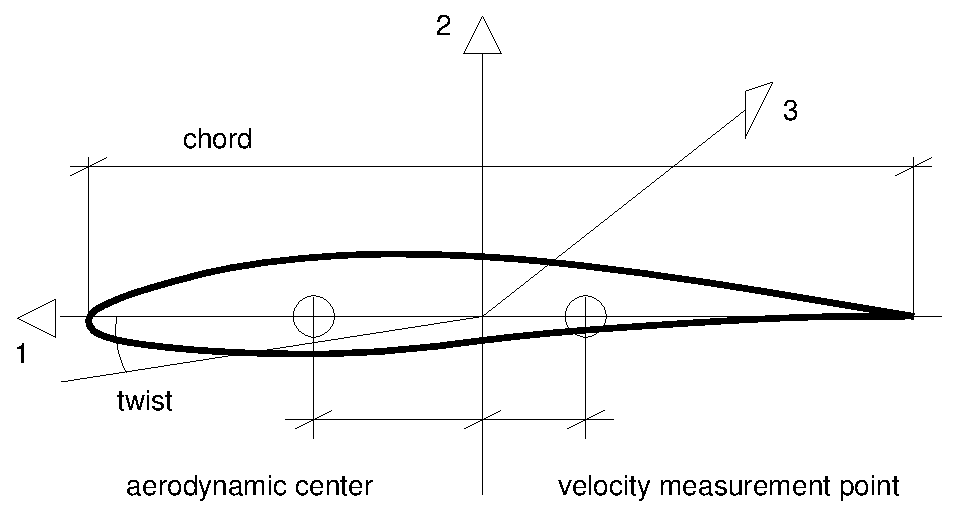
\includegraphics[width=80mm]{airfoil.eps}
  \caption{\em Airfoil Geometry}\label{fig:AIRFOIL}
\end{figure}


\subsection{Output}
Aerodynamic elements, both bodies and beams, write their output with file
extension {\tt .aer}; for each time step the required elements are output.
Three different formats are available; the format can be selected only at
compile time, and it must be the same for all the elements. 

\noindent
{\em Note: it will stabilize, eventually; if all the output formats will be
maintained, they will be made selectable at run-time.}

\noindent
In any case the label of the element is output first.

\subsubsection{Node}
The format is:
\begin{itemize}
    \item the label of the node
    \item the three components of the force applied to the node
    \item the three components of the couple applied to the node
\end{itemize}
When an aerodynamic beam is considered, the output is repeated for each node
the element is attached to.

\subsubsection{Gauss --- forces}
The output refers to each Gauss integration point; the format is:
\begin{itemize}
    \item the direction of the wind velocity relative to the element frame
    \item the lift,
    \item the drag,
    \item and the aerodynamic moment per unit length
\end{itemize}
When an aerodynamic beam is considered, the output is repeated for each
portion of beam.

\subsubsection{Gauss --- properties}
The output refers to each Gauss integration point; the format is:
\begin{itemize}
    \item the local incidence
    \item the local yaw angle
    \item the local mach number
    \item the lift,
    \item the drag,
    \item and the aerodynamic moment per unit length
\end{itemize}
When an aerodynamic beam is considered, the output is repeated for each
portion of beam.






\section{Air Properties Element}
\begin{verbatim}
    <arglist> ::= (scalar) <air_density> , 
                  (scalar) <sound_speed> ,
                  (Vec3_tpl_drive_caller) <air_speed>
\end{verbatim}
the asymptotic air properties are characterised by the drive of the 
air speed, in the global reference frame.





\section{Beam Element}
Currently two beam elements are implemented: a three-node finite volume
element, which has been historically implemented first, which uses
conventional polynomial parabolic interpolation of the nodal displacements
and rotations, and a two-node finite volume element, which has been
recently introduced.
Although this latter element presents some shear-locking, it may be overcome
by correcting the section stiffness matrix in a straightforward form:
\begin{displaymath}
	\hat{K} \ = \ \plbr{F + \frac{L^2}{12}T F T^T}^{-1} ,
\end{displaymath}
where $F=K^{-1}$ is the compliance of the section, and
\begin{displaymath}
	T \ = \ sqbr{\matr{cc}{
		0 & e_x \times{} \\
		0 & 0
	}}
\end{displaymath}
is the ``arm'' matrix that appears in the differential equilibrium equation
\begin{displaymath}
	\vartheta_{/x} - T^T\vartheta + f \ = \ 0 .
\end{displaymath}
The two-node beam will be reimplemented using helicoidal interpolation
of the nodal displacements and rotations, to reduce the shear-locking effect.

\subsection{Three-node beam element}
The beam element is a three node one-dimensional element.
Each ``node'' is referred to a structural node but can have an arbitrary
offset to allow for more generality in positioning of the structural 
reference lines of the beam.
The ``Finite Volumes'' formulation is used. 
This implies the evaluation of the internal forces at two points 
that are close to the middle point between nodes 1 and 2, 
and between nodes 2 and 3 (at $ 1-1/\sqrt{3} $ from both ends).
So the constitutive properties must be supplied in these points, as well as
the rotation matrices from the material to the global frame (the axial force
is in direction 1).
Any of the allowed 6D constitutive laws can be supplied to define the
constitutive properties.
\begin{verbatim}
    <element_type> ::= beam
    <normal_arglist> ::=
        <node_1> , (Vec3) <relative_offset_1> ,
        <node_2> , (Vec3) <relative_offset_2> ,
        <node_3> , (Vec3) <relative_offset_3> ,
        (RotationMatrix) <rotation_matrix_section_I> ,
        (ConstitutiveLaw6D) <constitutive_law_section_I> ,
        (RotationMatrix) <rotation_matrix_section_II> ,
        (ConstitutiveLaw6D) <constitutive_law_section_II>
\end{verbatim}
Based on the type of constitutive law, the simple or the viscoelastic beam
element is used. \\
A piezoelectric actuator beam element is available; an arbitrary
linear piezoelectric actuation matrix is required, together with the labels
of the abstract nodes that represent the input signal tensions, as follows:
\begin{verbatim}
    <normal_arglist> ::=
        <node_1> , (Vec3) <relative_offset_1> ,
        <node_2> , (Vec3) <relative_offset_2> ,
        <node_3> , (Vec3) <relative_offset_3> ,
        (RotationMatrix) <rotation_matrix_section_I> ,
        (ConstitutiveLaw6D) <constitutive_law_section_I> ,
        (RotationMatrix) <rotation_matrix_section_II> ,
        (ConstitutiveLaw6D) <constitutive_law_section_II>
        piezoelectric actuator , 
        <electrodes_number> ,
        <abstract_node_label_list> ,
        (Mat6xN) <piezoelectric_matrix_I> ,
        { same | (Mat6xN) <piezoelectric_matrix_II> }
\end{verbatim}
where the {\tt abstract\_node\_label\_list} is the list of the labels of the
abstract nodes that represent the electrodes.

\subsection{Two-node beam element}
\begin{verbatim}
    <element_type> ::= beam2
    <normal_arglist> ::=
        <node_1> , (Vec3) <relative_offset_1> ,
        <node_2> , (Vec3) <relative_offset_2> ,
        (RotationMatrix) <rotation_matrix_section_I> ,
        (ConstitutiveLaw6D) <constitutive_law_section_I>
        [ , piezoelectric actuator , 
        <electrodes_number> ,
        <abstract_node_label_list> ,
        (Mat6xN) <piezoelectric_matrix_I> ]
\end{verbatim}

\subsection{Output}
The output related to beam elements is contained in a file with extension 
{\tt .act}; for each time step, the output of thre required beams is
considered.
The internal forces and couples are computed from the interpolated strains
along the beam by means of the constitutive law, at the two evaluation
points. 
The format is:
\begin{itemize}
    \item the label of the beam
    \item the three components of the force at the first evaluation point
    \item the three components of the couple at the first evaluation point
    \item the three components of the force at the second evaluation point
    \item the three components of the couple at the second evaluation point    
\end{itemize}



\section{Bind}\label{sec:EL-BIND}
This is not really an element; it is used to instruct a {\tt parameter node}
about which parameter of an element it is bound to.
The {\tt parameter node} must exist, and the binding element, of type 
{\tt element\_type} and label {\tt element\_label}, must have been already 
defined.
The complete syntax is:
\begin{verbatim}
    <arglist> ::= <element_label> , 
                  <element_type> ,
                  <parameter_node_label> , 
                  <parameter_index>
\end{verbatim}
Each element makes a number of parameters available for such binding; a
detailed list will be presented in a future release of the input manual.
The value of {\tt parameter\_index} must be legal, i.e.\ between 1 and the
maximum number of parameters made available by the element.




\section{Body}
\begin{verbatim}
    <normal_arglist> ::= <node_label> , 
    { 
      (scalar) <mass> , 
      (Vec3)   <relative_center_of_mass> ,
      (Mat3x3) <inertia_matrix>
      [ , inertial , 
          { node | (RotationMatrix) <rotation_matrix> } ]
    |
      condense, (integer) <num_masses> ,
          (scalar) <mass> , 
          (Vec3)   <relative_center_of_mass> ,
          (Mat3x3) <inertia_matrix> 
          [ , inertial , 
              { node | (RotationMatrix) <rotation_matrix> } ]
          [ , ... ]
    }
\end{verbatim}
the {\tt inertia\_matrix} is always referred to the center of mass of the
mass that is being added. It can be rotated locally by means of the extra
{\tt rotation\_matrix} supplied after the (optional) keyword {\tt inertial}.
Otherwise, if the keyword {\tt node} is supplied after the keyword 
{\tt inertial}, the inertia matrix is not rotated at all, since it is
assumed to be already in the node reference frame.
If only one mass is defined, the first method should be used. Otherwise,
many masses can be referred to the same element by means of the keyword
{\tt condense}, followed by the number of expected masses {\tt num\_masses}.
The format of each submass is the same as for the single mass input (actually, 
when {\tt condense} is not supplied, {\tt num\_masses} is assumed to be 1).




\section{Bulk Elements}
The {\tt bulk} element is intended as a sort of NASTRAN's {\tt CELAS} card,
that can be used to apply a stiffness term on an arbitrary degree of freedom.
Extensions are planned to different kind of elements.
The syntax of the {\tt bulk} element is:
\begin{verbatim}
    <normal_arglist> ::= <bulk_type> , <bulk_arglist>
\end{verbatim}
At present only the {\tt stiffness spring} type is available.

\subsection{Stiffness spring}
\begin{verbatim}
    <bulk_type> ::= stiffness spring
    <bulk_arglist> ::= (node_dof) <dof> ,
                       (drive_caller) <stiffness_drive>
\end{verbatim}
The equation related to the desired dof of the linked node is added a
contribution based on the value of the desired degree of freedom (even the
derivative can be used) multiplied times the stiffness. \\
{\em Note: this family of elements has been partially superseeded by the
{\tt genel} elements, which allow more generality.}




\section{Driven Element}
The {\tt driven} type is not an element by itself. It is a wrapper that
masks another element and switches it on and off depending on the (boolean)
value of a drive. It can be used to emulate a variable topology model, where 
some elements simply don't contribute to the residuial or to the jacobian
matrices when their drive has a certain value. Since the drivers can be
arbitrary functions of the time, or other parameters including the value of
any degree of freedom, the driven elements can be ``driven'' in a very
flexible way. Every element can be driven, except those that can be
instantiated once only.
The syntax for a driven element is:
\begin{verbatim}
    <normal_arglist> ::= (drive_caller) <element_driver> ,
        {
            <elem_type> : <elem_label> <elem_normal_arglist> 
        |   
            existing : <elem_type> , <elem_label>
        }
\end{verbatim}
When the first format is used, a normal element is read, instantiated, and
wrapped by the {\tt driven} element wrapper. Note that after the element type,
or after the keyword {\tt existing}, a colon is used as a separator.
This is due for compatibility with the restart module and is not likely 
to be eliminated in the future. 
The label of the element must math that of the driving element given at
the beginning.
When the second format is used, an existing element is sought, and it is
wrapped by a driven element. In this case, no new element is instantiated.
Again the label of the element must match that of the driving element given 
at the beginning. For consistency with the syntax, and for more flexibility,
even when wrapping an existing element it is possible to set at the end the
output flags. This flag will override the previously set one.





\section{Electric Elements}
{\tt electric} elements are those elements that model electric and electronic
devices, dealing with abstract degrees of freedom more than with electric
ones (from the program's point of view they are exactly the same, the
difference is only semantic). The true electric elements, such resistors,
switches and so on, are clessified as {\tt electric bulk} elements.
The syntax for {\tt electric} elements is:
\begin{verbatim}
    <normal_arglist> ::= <electric_type> , <electric_arglist>
\end{verbatim}
The {\tt electric} elements implemented at present are:

\subsection{Accelerometer}
  \begin{verbatim}
    <electric_arglist> ::= <struct_node_label> ,
        <abstract_node_label> ,
        (Vec3) <measure_direction> ,
        (scalar) <omega> ,
        (scalar) <tau> ,
        (scalar) <csi> ,
        (scalar) <kappa>	
  \end{verbatim}
  The label {\tt struct\_node\_label} defines the node whose acceleration 
  is being measured; the label {\tt abstract\_node\_label} defines the
  {\tt abstract node} that will receive the output signal. 
  An {\tt electric node} can be used as well (?).
  The transfer function of the accelerometer is:
  \begin{displaymath}
    \frac{e_0}{a} = {\tt kappa}\frac{{\tt tau} \ s}{
      \plbr{1+{\tt tau} \ s}
      \plbr{1+2 \ {\tt csi}/{\tt omega} \ s+s^2/{\tt omega}^2}
    }
  \end{displaymath}
  where $ e_0 $ is the output signal, $ a $ is the input (the acceleration)
  and $ s $ is the Laplace variable.

\subsection{Discrete control}
  \begin{verbatim}
    <electric_arglist> ::= <num_outputs> , <num_inputs> , <order> ,
        <control_data> , 
        outputs [ , (node_dof) <output_dofs> [ , ... ] ] ,
        inputs [ , (node_dof) <input_dofs> [ , ... ] ] ,
  \end{verbatim}
  The lists of the output and input dofs follows. The input {\tt
  node\_dof}s don't require the {\tt order} field, since they are simply
  used to compute the control forces, and thus identify an equation.
  The {\tt control\_data} has the following syntax:
  \begin{verbatim}  
        <control_data> ::= <control_type> , <control_arglist>
  \end{verbatim}
  At present only a simple form of control is implemented. Other types
  to come are system identification, both recursive and one-shot, and
  adaptive control, with different models and schemes, all based on 
  Generalised Predictive Control (GPC) and Deadbeat Control.
  The {\tt control} syntax is:
  \begin{verbatim}
    <control_data> ::= control , " <control_matrices_file> "
  \end{verbatim}
  where the file {\tt control\_matrices\_file} must contain the matrices
  $ a_c $, $ b_c $ of the control in plain text (as generated by Matlab, for
  instance): \\
  \begin{tabular}{l}
    $ a_{c1} $, \\
    \ldots,     \\
    $ a_{cp} $, \\
    $ b_{c1} $, \\
    \ldots,     \\
    $ b_{cp} $  \\
  \end{tabular} \\
  where $ p $ is the {\tt order} of the controller and the matrices $ a_c $
  have {\tt num\_inputs} rows and {\tt num\_outputs} columns, while the
  matrices $ b_c $ have {\tt num\_inputs} rows and {\tt num\_inputs} columns.





\section{Force and Couple Elements}
The {\tt force} element has the following syntax:
\begin{verbatim}
  <normal_arglist> ::= <force_type> , <force_arglist>
\end{verbatim}
where {\tt <force\_type>} can be {\tt abstract} for an abstract force, or 
{\tt conservative} or {\tt follower} for a structural force. The latter types
apply to a {\tt couple} element, which can be structural only.

\subsection{Output}
The output is discussed accordingly to the types of forces. 
The label of the element is output first in all the cases.

\subsection{Abstract force}
\begin{verbatim}
    <force_type> ::= abstract 
    <force_arglist> ::= (node_dof) <dof> ,
                        (drive_caller) <force_magnitude>
\end{verbatim}
the {\tt dof} field is a normal {\tt node\_dof} but no {\tt order} is required
since the {\tt force} simply applies to the equation related to the node,
regardless of the order.

\subsubsection{Output}
The format is:
\begin{itemize}
    \item the label of the element
    \item the label of the abstract node the force is applied to
    \item the value of the force
\end{itemize}


\subsection{Structural force}
\begin{verbatim}
    <force_type> ::= { conservative | follower } 
    <force_arglist> ::= <node> , 
                        (Vec3) <relative_direction> ,
                        (Vec3) <relative_arm> ,
                        (drive_caller) <force_magnitude>
\end{verbatim}

\subsubsection{Output}
The format is:
\begin{itemize}
    \item the label of the element
    \item the label of the structural node the force is applied to
    \item the value of the force
    \item the three components of the force
    \item the arm of the force, in the global frame (i.e.\ referred
          to point $ \cubr{0,0,0} $)
\end{itemize}


\subsection{Structural couple}
\begin{verbatim}
    <force_type> ::= { conservative | follower } 
    <force_arglist> ::= <node> ,
                        (Vec3) <relative_direction> ,  
                        (drive_caller) <couple_magnitude>
\end{verbatim}
i.e.\ the arm is not required. 

\subsubsection{Output}
The format is:
\begin{itemize}
    \item the label of the element
    \item the label of the structural node the couple is applied to
    \item the value of the couple
    \item the three components of the couple
\end{itemize}


\noindent
{\em 
Note: by using a {\tt dof} drive, a simple feedback control can be easily
implemented. \\
A more general force element can be written by using a template drive
that contains both the direction and the amplitude. This will be done in the
future. 
}





\section{Genel Element}
{\sc Genel} is the compact form for {\sc \bf Gen}eral {\sc el}ement. Those
elements cannot in general be classified in a precise way, or are just
under development and thus are not collected in a class of their own until
their configuration is stabilized. 
The syntax of the {\sc Genel} elements is:
\begin{verbatim}
    <normal_arglist> ::= <genel_type> , <genel_arglist>
\end{verbatim}

\noindent
The output goes in a file with extension {\tt .gen}; only few elements
actually generate output.

\noindent
At present there are very simple {\sc Genel}
elements, plus a very particular one, that is the {\tt swash plate}.
It is used to transform the controls of a rotor, in terms of collective
and fore/aft and lateral cyclic pitch, into the elongations of the actuators 
that actually move the swash plate.
The syntax of the {\tt genel}s is:

\subsection{Swashplate}
\begin{verbatim}
    <genel_type> ::= swash plate
    <genel_arglist> ::=
        <collective_abstract_node> 
        [ , limits , <min_collective> , <max_collective> ] ,
        <fore/aft_abstract_node> 
        [ , limits , <min_fore/aft> , <max_fore/aft> ] ,
        <lateral_abstract_node> 
        [ , limits , <min_lateral> , <max_lateral> ] ,
        <actuator_1_abstract_node> ,
        <actuator_2_abstract_node> ,
        <actuator_3_abstract_node> 
        [ , <dynamic_coef> , <cyclic_factor> , <collective_factor> ]
\end{verbatim}
The first three abstract nodes will contain the input values (they can be
actuated by means of abstract forces), and the limits on the ``angles'' can
be easily set. 
The last three nodes will contain the values of the stroke of the actuators.
It is assumed that one of the actuators is behind and the others two are in
front of the rotor, numbered clockwise from the top. 
The limits on the actuators will simply force the value of the control
inputs to remain in the boundaries regardless of the input values.
The last three optional parameters are a dynamic coefficient that is used to
add some dynamics to the actuators' stroke, namely the input variables are
applied a sort of {\tt spring stiffness} {\tt bulk} element, while the
actuators' strokes are applied a transfer function of the first order, namely
$ \alpha\dot{x}+x=f $, where $ \alpha={\tt dynamic\_coef} $ and $ f $ is
the desired stroke, so the smaller is $ \alpha $, the more the behaviour is
static.
The {\tt cyclic\_factor} and the {\tt collective\_factor} parameters are
used to scale the inputs from angles in the desired units to strokes, that
usually are dimensional parameters. The actual strokes are made of the
collective contribution multiplied by {\tt collective\_factor}, and the
cyclic contribution multiplied by {\tt collective\_factor} times 
{\tt cyclic\_factor}.
   
\subsection{Clamp}
\begin{verbatim}
    <genel_type> ::= clamp
    <genel_arglist> ::= (node_dof) <clamped_node> ,
                        (drive_caller) <imposed_value>
\end{verbatim}
This element simply forces one arbitrary degree of freedom to assume a value
depending on the drive.

\paragraph{Output}
The format is:
\begin{itemize}
    \item the label of the element
    \item the value of the reaction unknown
\end{itemize}
  
\subsection{Distance}
\begin{verbatim}
    <genel_type> ::= distance
    <genel_arglist> ::= (node_dof) <node_1> ,
                        (node_dof) <node_2> ,
                        (drive_caller) <imposed_distance>
\end{verbatim}
This element forces the difference between two arbitrary degrees of freedom
to assume the value dictated by the driver.

\paragraph{Output}
The format is:
\begin{itemize}
    \item the label of the element
    \item the value of the reaction unknown
\end{itemize}
  
  
\subsection{Spring}
\begin{verbatim}
    <genel_type> ::= spring
    <genel_arglist> ::= (node_dof) <node_1> ,
                        (node_dof) <node_2> ,
                        (ConstitutiveLaw1D) <const_law>
\end{verbatim}
{\em 
    Note: the constitutive law must be {\tt elastic}, but the {\tt distance}
    genel can apply to arbitrary order degrees of freedom, even between degrees 
    of freedom of different order.
}

\subsection{Spring support}
\begin{verbatim}
    <genel_type> ::= spring support
    <genel_arglist> ::= (node_dof) <node> ,                      
                        (ConstitutiveLaw1D) <const_law>
\end{verbatim}
{\em
    Note: the {\tt spring support} must use the {\tt algebraic} value of a 
    {\tt differential} node, but it can use an arbitrary constitutive law,
    i.e.\ an elastic constitutive law for a spring, or a viscous
    constitutive law for a damper, and so on.
}

\subsection{Cross spring support}
\begin{verbatim}
    <genel_type> ::= spring support
    <genel_arglist> ::= (node_dof) <row_node> ,                      
                        (node_dof) <col_node> ,                      
                        (ConstitutiveLaw1D) <const_law>
\end{verbatim}
It writes a term depending on the {\tt col\_node} degree of freedom in an
arbitrary manner (given by the {\tt const\_law}) to the 
{\tt row\_node} equation. \\
{\em
    Note: the {\tt cross spring support} must use the {\tt algebraic} value
    of a {\tt differential} node, but can use an arbitrary constitutive law,
    i.e.\ an elastic constitutive law for a spring, or a viscous
    constitutive law for a damper, and so on.
}

\subsection{Mass}
\begin{verbatim}
    <genel_type> ::= mass
    <genel_arglist> ::= (node_dof) <node> ,                     
                        (drive_caller) <mass>
\end{verbatim}
{\em
    Note: the mass must use the {\tt algebraic} value of a {\tt
    differential} node. The derivative of the {\tt differential} value of
    the dof is differentiated in a state-space sense, and an inertial driven
    term is applied to the equation related to the dof:
    \begin{eqnarray*}
        m\dot{u} + \ldots & = & f \\
	u - \dot{x} & = & 0
    \end{eqnarray*}
}

\subsection{Scalar filter}
\begin{verbatim}
    <genel_type> ::= scalar filter
    <genel_arglist> ::= (node_dof) <output_node> ,
                        (node_dof) <input_node> ,
                        <output_order> [ , <output_coef_list> ] ,
                        <input_order> , <input_coef_list>
                        [ , gain , <gain> ]
\end{verbatim}
This element models a scalar filter of the form
\begin{displaymath}
    A\plbr{s}y = B\plbr{s}u
\end{displaymath}
where $ A $, $ B $ are polynomials of arbitrary order, provided it is
causal, namely the {\tt output\_order} is greater than or equal to 
the {\tt input\_order}.
The polynomial $ A $ is assumed to be monic, so only the coefficients
from 1 to {\tt output\_order} must be input, while all the coefficients 
of polynomial $ B $ are required, i.e.\ from 0 to {\tt input\_order}.
If a gain is supplied, all the coefficients of $ B $ are multiplied by the
gain.

\subsection{State space SISO}
\begin{verbatim}
    <genel_type> ::= state space SISO
    <genel_arglist> ::= (node_dof) <output_node> ,
                        (node_dof) <input_node> ,
                        <state_order> ,
                        matrix A , <coefficient_list> ,
                        matrix B , <coefficient_list> ,
                        matrix C , <coefficient_list>
                        [ , matrix D , <coefficient> ]
\end{verbatim}
This element models a scalar (SISO) state space filter of the form
\begin{displaymath}
    \lvvect{ 
        \dot{x} = Ax+Bu \\
	y = Cx+Dx
    }
\end{displaymath}
where $ A $ is a matrix {\tt state\_order}$\times${\tt state\_order},
$ B $ is a vector {\tt state\_order}$\times$1,
$ C $ is a vector 1$\times${\tt state\_order},
and $ D $ is scalar, if any.
The matrices are read row-oriented.

\subsection{State space MIMO}
\begin{verbatim}
    <genel_type> ::= state space MIMO
    <genel_arglist> ::= <num_outputs> , (node_dof) <output_node_list> ,
                        <num_inputs> , (node_dof) <input_node_list> ,
                        <state_order> ,
                        matrix A , <coefficient_list> ,
                        matrix B , <coefficient_list> ,
                        matrix C , <coefficient_list>
                        [ , matrix D , <coefficient_list> ]
\end{verbatim}
This element models a scalar (SISO) state space filter of the form
\begin{displaymath}
    \lvvect{ 
        \dot{x} = Ax+Bu \\
	y = Cx+Dx
    }
\end{displaymath}
where $ A $ is a matrix {\tt state\_order}$\times${\tt state\_order},
$ B $ is a matrix {\tt state\_order}$\times${\tt num\_inputs},
$ C $ is a matrix {\tt num\_outputs}$\times${\tt state\_order},
and $ D $ is scalar {\tt num\_outputs}$\times${\tt num\_inputs}.
The matrices are read row-oriented.




\section{Gravity Element}
\begin{verbatim}
    <arglist> ::= (Vec3_tpl_drive_caller) <gravity_acceleration>
\end{verbatim}
the drive of the gravity acceleration, in the global reference frame.




\section{Hydraulic Element}\label{sec:HYDRAULIC-ELEMENT}
{\em 
    Note: under development \\
    Author: Lamberto Puggelli
}
\begin{verbatim}
    <normal_arglist> ::= <hydr_elem_type> , 
                         <hydr_elem_data>
\end{verbatim}
A detailed input description will be given as soon as it is available. \\
{\tt hydraulic\_element\_data} usually contains information about fluid
properties, which are handled by means of an {\tt hydraulic\_fluid}.
This can be directly inserted, following the syntax described in
Section~\ref{sec:HYDRAULIC-FLUID} preceeded by the keyword {\tt fluid}, or a
previously defined fluid can be recalled by using the keyword 
{\tt reference} followed by the label of the desired fluid.

\subsection{Actuator}
\begin{verbatim}
    <hydr_elem_type> ::= actuator ,
    <hydr_elem_data> ::= <node_1> , <node_2> , 
                         <struct_node_1> , (Vec3) <offset_1> ,
                         <struct_node_2> , (Vec3) <offset_2> ,
                         [ direction , (Vec3) <direction> , ]
                         <area_1> ,
                         <area_2> ,
                         <cylinder_length> ,
                         <hydraulic_fluid_properties_1> ,
                         { same | <hydraulic_fluid_properties_2> }
\end{verbatim}

\subsection{Minor Loss}
\begin{verbatim}
    <hydr_elem_type> ::= minor loss ,
    <hydr_elem_data> ::= <node_1> , <node_2> ,
                         <k12> , <k21> , <area> ,
                         <hydraulic_fluid_properties>
\end{verbatim}

\subsection{Control Valve}
\begin{verbatim}
    <hydr_elem_type> ::= control valve ,
    <hydr_elem_data> ::= <node_1> , <node_2> , <node_3> , <node_4>
                         <area> ,
                         [ loss , <loss_factor> , ]
                         (DriveCaller) <state> ,
                         <hydraulic_fluid_properties>
\end{verbatim}
This element represrents a valve that connects
{\tt node\_1} to {\tt node\_2} and {\tt node\_3} to {\tt node\_4}
when {\tt state} is positive and {\tt node\_1} to {\tt node\_3}
and {\tt node\_2} to {\tt node\_4} when {\tt state} is negative,
with area proportional to {\tt area} times the norm of {\tt state}, 
being the latter comprised between $-1$ and $1$.
If {\tt loss\_factor} is defined, it represents the fraction
of area that leaks even when {\tt state} is zero.



\subsection{Dynamic Control Valve}\label{sec:DYNAMIC_CONTROL_VALVE}
\begin{verbatim}
    <hydr_elem_type> ::= dynamic control valve ,
    <hydr_elem_data> ::= <node_1> , <node_2> ,
                         <node_3> , <node_4> ,
                         (DriveCaller) <force> ,
                         <initial_displacement> ,
                         <max_displacement> ,
                         <duct_width> ,
                         [ loss , <loss_factor> , ]
                         <valve_diameter> ,
                         <valve_density> ,
                         <displacement> ,
                         <velocity> ,
                         <acceleration> ,
                         <hydraulic_fluid_properties>
\end{verbatim}
This element represrents a valve that connects
{\tt node\_1} to {\tt node\_2} and {\tt node\_3} to {\tt node\_4}
when the displacement is positive and {\tt node\_1} to {\tt node\_3}
and {\tt node\_2} to {\tt node\_4} when the displacement is negative,
accounting for the dynamics of the valve body.
The control force {\tt force} is applied to the valve, whose 
geometric and structural properties are described by 
{\tt initial\_displacement}, {\tt max\_displacement},
{\tt duct\_width}, {\tt valve\_diameter} and {\tt valve\_density}.
Again the {\tt loss\_factor}, if defined, represents the fraction
of the area that leaks when the displacement is zero.
Finally, {\tt displacement}, {\tt velocity} and {\tt acceleration}
are the penalty coefficients for displacement, valocity and acceleration
when the maximum stroke is reached.




\subsection{Pressure Flow Control Valve}
\begin{verbatim}
    <hydr_elem_type> ::= pressure flow control valve ,
    <hydr_elem_data> ::= <node_1> , <node_2> ,
                         <node_3> , <node_4> ,
                         <node_5> , <node_6> ,
                         (DriveCaller) <force> ,
                         <initial_displacement> ,
                         <max_displacement> ,
                         <duct_width> ,
                         [ loss , <loss_factor> , ]
                         <valve_diameter> ,
                         <valve_density> ,
                         <displacement> ,
                         <velocity> ,
                         <acceleration> ,
                         <hydraulic_fluid_properties>
\end{verbatim}
Same as Dynamic Control Valve (\ref{sec:DYNAMIC_CONTROL_VALVE}),
only the pressures at {\tt node\_5} and {\tt node\_6} are applied
at the sides of the valve body and participate in the force balance.



\section{Joint Element}
Many different joints are available. A first rough classification can be
based on which joints have internal degrees of freedom (the reactions) and
which don't. The latter are flexible joints, that directly add their
stiffness contribution to the dynamic system matrix. From the input point
of view there is no difference between the two classes.
a typical joint entry is made as follows:
\begin{verbatim}
    <normal_arglist> :: = <joint_type> , <joint_arglist>
\end{verbatim}
The output is written to a file with extension {\tt .jnt}.
The output is generally made of a standard part, plus some extra information
depending on the type of joint, which, when available, is described along
with the joint description.
Here the standard part is described:
\begin{itemize}
    \item the label of the joint
    \item the three components of the reaction force in a local reference
    \item the three components of the reaction couple in a local frame
    \item the three components of the reaction force in the global frame
    \item the three components of the reaction couple, rotated into the
          global frame
\end{itemize}
Legal joint types, with relative data, are:


\subsection{Distance}
\begin{verbatim}
    <joint_type> ::= distance 
    <joint_arglist> ::= <node_1> , <node_2> ,
                        { (drive_caller) <distance> | from nodes }
\end{verbatim}

\noindent
{\em
    Note: in case the keywords {\tt from nodes} are used, a constant drive
    caller is automatically instantiated for the {\tt distance}. 
    Its value is computed from the initial positions of the nodes.
}

\paragraph{Output}
The extra output is:
\begin{itemize}
    \item the three components of the imposed distance in the global frame
    \item the norm of the imposed distance
\end{itemize}


\subsection{Distance with offset}
\begin{verbatim}
    <joint_type> ::= distance with offset
    <joint_arglist> ::= <node_1> , (Vec3) <relative_offset_1> ,
                        <node_2> , (Vec3) <relative_offset_2> , 
                        { (drive_caller) <distance> | from nodes }
\end{verbatim}
{\em 
    Note: the {\tt relative\_offset\_*} are the distances of each end
    of the joint from the relative nodes in the node reference frame \\
    Both the {\tt distance} and the {\tt distance with offset} joints
    allow for null distance, but the transition from null to non-null
    distance is not smooth at all.
} \\
{\em
    Note: in case of {\tt from nodes}, the same stated for the {\tt distance}
    joint applies, except that the distance between the offsets is
    considered. 
}

\subsection{Clamp}
\begin{verbatim}
    <joint_type> ::= clamp 
    <joint_arglist> ::= <node> , 
        { node | (Vec3) <absolute_position> } ,
        { node | (RotationMatrix) <absolute_rotation_matrix> }
\end{verbatim}
{\em
    Note: the keyword {\tt node} forces the joint to use the nodal position
    and reference frame. Otherwise, they must be entered in the usual way
    for these entities
}

\subsection{Coincidence}
not implemented yet, use a {\tt spherical hinge} and a {\tt prismatic} 
instead.

\subsection{Spherical hinge}
\begin{verbatim}
    <joint_type> ::= spherical hinge
    <joint_arglist> ::= 
        <node_1> , (Vec3) <relative_offset_1> 
        [ , hinge , 
            (RotationMatrix) <relative_rotation_matrix_1> ] ,
        <node_2> , (Vec3) <relative_offset_2>
        [ , hinge , 
            (RotationMatrix) <relative_rotation_matrix_2> ]
\end{verbatim}
{\em
    Note: the rotation matrix is used for output purposes only. 
    A default identity matrix is assumed.
}

\subsection{Pin}
\begin{verbatim}
    <joint_type> ::= pin
    <joint_arglist> ::= <node> , (Vec3) <relative_offset> ,
                                 (Vec3) <absolute_pin_position>
\end{verbatim}
{\em
    Note: this is the dual of the spherical hinge when one node is grounded.
    An alternative way to model a grounded spherical hinge requires the use
    of a static, clamped node.
}

\subsection{Universal hinge}
\begin{verbatim}
    <joint_type> ::= universal hinge
    <joint_arglist> ::= 
        <node_1> , (Vec3) <relative_offset_1> 
        [ , hinge , 
            (RotationMatrix) <relative_rotation_matrix_1> ] ,
        <node_2> , (Vec3) <relative_offset_2>
        [ , hinge , 
            (RotationMatrix) <relative_rotation_matrix_2> ]
\end{verbatim}
{\em
    Note: this joint forces the relative direction 3 of node 1 to be always 
    normal to the relative direction 2 of node 2.
}

\subsection{Universal pin}
\begin{verbatim}
    <joint_type> ::= universal pin
    <joint_arglist> ::= 
        <node> , (Vec3) <relative_offset>
        [ , hinge , 
            (RotationMatrix) <relative_rotation_matrix> ] ,
        (Vec3) <absolute_pin_position>
        [ , hinge , 
            (RotationMatrix) <absolute_pin_rotation_matrix> ]
\end{verbatim}
{\em
    Note: this is the dual of the universal hinge when one node is grounded.
}

\subsection{Plane hinge}
\begin{verbatim}
    <joint_type> ::= plane hinge
    <joint_arglist> ::= 
        <node_1> , (Vec3) <relative_offset_1> 
        [ , hinge , 
            (RotationMatrix) <relative_rotation_matrix_1> ] ,
        <node_2> , (Vec3) <relative_offset_2>
        [ , hinge , 
            (RotationMatrix) <relative_rotation_matrix_2> ]
\end{verbatim}
{\em
    Note: this joint forces nodes 1 and 2 to rotate only about relative 
    axis 3.
}

\subsection{Plane pin}
\begin{verbatim}
    <joint_type> ::= plane pin
    <joint_arglist> ::= 
        <node> , (Vec3) <relative_offset>
        [ , hinge , 
            (RotationMatrix) <relative_rotation_matrix> ] ,
        (Vec3) <absolute_pin_position>
        [ , hinge , 
            (RotationMatrix) <absolute_pin_rotation_matrix> ]
\end{verbatim}
{\em
    Note: this is the dual of the plane hinge when one node is grounded.
}

\subsection{Axial rotation}
\begin{verbatim}
    <joint_type> ::= axial rotation
    <joint_arglist> ::= 
        <node_1> , (Vec3) <relative_offset_1> 
        [ , hinge , 
            (RotationMatrix) <relative_rotation_matrix_1> ] ,
        <node_2> , (Vec3) <relative_offset_2>
        [ , hinge , 
            (RotationMatrix) <relative_rotation_matrix_2> ] ,
        (drive_caller) <angular_velocity>
\end{verbatim}
{\em
    Note: this joint forces nodes 1 and 2 to rotate about relative 
    axis 3 with imposed angular velocity.
}

\subsection{In plane}
\begin{verbatim}
    <joint_type> ::= in plane
    <joint_arglist> ::= 
        <node_1> , 
        (Vec3) <relative_plane_position> ,
        (Vec3) <relative_normal_direction> ,
        <node_2>
        [ , offset , (Vec3) <relative_offset>]
\end{verbatim}
{\em
    Note: to make an in-line joint, use two in-plane joints, with the
    planes that intersect along the desired line. \\
    Note: a {\tt inline} element has been added, which automates the above
    reported procedure.
}

\subsection{In line}
\begin{verbatim}
    <joint_type> ::= in line
    <joint_arglist> ::= 
        <node_1> , 
        (Vec3) <relative_line_position> ,
        (Mat3x3) <relative_orientation> ,
        <node_2>
        [ , offset , (Vec3) <relative_offset>]
\end{verbatim}
{\em 
    Note: the {\tt in line} joint supersedes the former note; the orientation
    assumes the sliding line is in direction 3.
}

\subsection{Rod}
\begin{verbatim}
    <joint_type> ::= rod 
    <joint_arglist> ::= <node_1> , <node_2> , 
        (scalar) { <rod_length> | from nodes }
        [ , offset , (Vec3) <relative_offset_1> , 
                     (Vec3) <relative_offset_2> ] ,
        (ConstitutiveLaw1D) <const_law>
\end{verbatim}

\subsection{Rod with offset}
\begin{verbatim}
    <joint_type> ::= rod with offset
    <joint_arglist> ::= <node_1> , (Vec3) <relative_offset_1>
                        <node_2> , (Vec3) <relative_offset_2>
        (scalar) { <rod_length> | from nodes } ,
        (ConstitutiveLaw1D) <const_law>
\end{verbatim}
Analogous to {\tt rod} with the optional arg {\tt offset}.    

\subsection{Deformable hinge}
\begin{verbatim}
    <joint_type> ::= deformable hinge
    <joint_arglist> ::= 
        <node_1>
        [ , hinge , (RotationMatrix) <relative_rotation_matrix_1> ] ,
        <node_2> 
        [ , hinge , (RotationMatrix) <relative_rotation_matrix_2> ] ,
        (ConstitutiveLaw3D) <const_law>
\end{verbatim}
{\em 
    Note: this hinge constrains the rotations only.
    It should be used in conjunction with a spherical hinge or any kind of
    joint that constrains the displacements too.
}

\subsection{Deformable displacement hinge}
\begin{verbatim}
    <joint_type> ::= deformable displacement hinge
    <joint_arglist> ::= 
        <node_1> , (Vec3) <relative_offset_1>
        [ , hinge , (RotationMatrix) <relative_rotation_matrix_1> ] ,
        <node_2> , (Vec3) <relative_offset_2>
        [ , hinge , (RotationMatrix) <relative_rotation_matrix_2> ] ,
        (ConstitutiveLaw3D) <const_law>
\end{verbatim}

\subsection{Linear velocity}
\begin{verbatim}
    <joint_type> ::= linear velocity
    <joint_arglist> ::= <node> , (Vec3) <relative_direction> , 
                        (drive_caller) <velocity>
\end{verbatim}

\subsection{Angular velocity}
\begin{verbatim}
    <joint_type> ::= angular velocity
    <joint_arglist> ::= <node> , (Vec3) <relative_direction> , 
                        (drive_caller) <velocity>
\end{verbatim}

\subsection{Linear acceleration}
\begin{verbatim}
    <joint_type> ::= linear acceleration
    <joint_arglist> ::= <node> , (Vec3) <relative_direction> , 
                        (drive_caller) <acceleration>
\end{verbatim}

\subsection{Angular acceleration}
\begin{verbatim}
    <joint_type> ::= angular acceleration
    <joint_arglist> ::= <node> , (Vec3) <relative_direction> , 
                        (drive_caller) <acceleration>
\end{verbatim}

\subsection{Prismatic}
\begin{verbatim}
    <joint_type> ::= prismatic
    <joint_arglist> ::= 
        <node_1>
        [ , hinge , (RotationMatrix) <relative_rotation_matrix_1> ] ,
        <node_2> 
        [ , hinge , (RotationMatrix) <relative_rotation_matrix_2> ] ,    
\end{verbatim}

\subsection{Drive hinge}
\begin{verbatim}
    <joint_type> ::= drive hinge
    <joint_arglist> ::= 
        <node_1>
        [ , hinge , (RotationMatrix) <relative_rotation_matrix_1> ] ,
        <node_2> 
        [ , hinge , (RotationMatrix) <relative_rotation_matrix_2> ] ,
        (Vec3_tpl_drive_caller) <hinge_rotation>
\end{verbatim}
{\em
    Note: this element is eXperimental. 
}
  
\subsection{Modal}\label{ELEMS-JOINT-MODAL}
{\em 
    Note: under development \\
    Author: Felice Felippone
}
\begin{verbatim}
    <joint_type> ::= modal
    <joint_arglist> ::= <reference_modal_node> ,
                        <mode_number> ,
                        <fem_node_number> 
                        [ , no damping 
                          | proportional damping , <damping_coef>
                          | diag damping , 
                            <mode_index> , <mode_damping_coef> 
                            [ , ... ] 
                        ] , " <fem_data_file> " ,
                        <interface_nodes_number> ,
                        <fem_node_label> , (Vec3)<offset> ,
                            <multibody_label> , (Vec3)<offset>
			[ , ... ] ,
                        " <output_file> "
\end{verbatim}
The {\tt reference\_modal\_node} is a special dynamic structural node that
is required to handle the rigid body motion of the modal joint.
Its input is completely analogous th that of the {\tt dynamic} structural
nodes, see Section~\ref{sec:NODE-STRUCT}, only the keyword {\tt dynamic} 
needs be replaced by {\tt modal}.
The format of the {\tt fem\_data\_file} is not documented yet.




\section{Loadable Element}
The {\tt loadable} element is a wrapper for a user-defined element that is
comipled in a separated module and linked run-time.
The module should provide a comprehensive set of functions with a specified
API; default functions are available if no special features are required.
Implementation of modules can be very easy, but a deep knowledge of the
internals of the code is required if special tasks are required. 
There are virtually no limits on what a loadable element can do.
The syntax is simply:
\begin{verbatim}
    <normal_arglist> ::= " <module_name> "
                         [ , name, " <calls> " ] 
                         [ , <module_data> ]
\end{verbatim}
where {\tt module\_name} is the name of the module file; as soon as the file
is checked and the binding of the structure with function bindings 
succeeded, a function called {\tt read} is invoked, and passed the input
stream.
This function is in charge of reading {\tt module\_data} following the
general syntax of the input file.
It is advisable that the function {\tt read} print some help message
when the first field of {\tt module\_data} is the keyword {\tt help}.
All the helpers and the high-level structures are available, such as
drivers, constitutive laws, reference frames.
Refer to each module for a description (if available) of the features and of
the input/output format.
{\tt module\_name} should be a full path to the module function.
If the name starts with a slash ``/'', the full path name is used.
Otherwise the module is searched in the colon-separated list of directories 
contained in the environment variable {\tt LD\_LIBRARY}, then among the
libraries listed in {\tt /etc/ld.so.cache}, and finally in
{\tt /usr/lib} and in {\tt /lib} (see {\tt dlopen(3)}).
At last, it is searched in the current directory, and the extension
{\tt .so} is added if missing.
The string {\tt calls} represents the name of the structure that contains
the bindings to the functions.
The default is {\tt "calls"}.
Refer to {\tt \$(BASE)/mbdyn/base/loadable.h} for a description of the
functions that are allowed.
An example module is given in directory
\begin{verbatim}
    $(BASE)/modules/module-template/
\end{verbatim}
which can be used as a starting point for building a custom module.
An analogous C/FORTRAN style interface is being planned, at the cost of
possibly losing some of the fancy C++ features made available by the code.





\section{Rotor Element}
The {\tt rotor} element is used to associate the aerodynamic elements that
model the blades of a rotor when some inflow related computations are
required. By means of different inflow models, and by means of the
aerodynamic load contributions supplied by the aerodynamic elements, the
rotor element is able to compute the induced velocity at an arbitrary point on
the rotor disk. This velocity term on turn is used by the aerodynamic
elements to determine a better estimate of the boundary conditions.
The syntax of the {\tt rotor} element is:
\begin{verbatim}
    <normal_arglist> ::= <craft_node> , <rotor_node> ,
        induced velocity : <ind_velocity>
\end{verbatim}
{\em 
    Note that after the keyword {\tt induced velocity}, a colon is used as a
    separator. This will probably be elminated in the future.
} \\
There are five models of induced velocity. 
The first is no induced velocity; the syntax is:
\begin{verbatim}
    <induced_velocity> ::= no
\end{verbatim}
There is no argument list. This element doesn't compute any induced
velocity, but still computes the rotor traction for output purposes.
The others have a fairly common syntax. The forst three are
{\tt uniform}, {\tt glauert} and {\tt mangler} induced velocity:
\begin{verbatim}
    <induced_velocity> ::= { uniform | glauert | mangler } , 
        <reference_omega> , <reference_radius> 
        [ , <memory_factor> ]
\end{verbatim}
the {\tt reference\_omega} field is used to decide wether to round off the
dimensionless parameters if the rotor speed is very low; the
{\tt reference\_radius} field is used in the adimensionalisation of the
rotor related parameters; the {\tt memory\_factor} parameter is used to
combine the current reference induced velocity with the induced velocity
at the previous step. It represents the weight that is given to the value at
the previous step; no weight means there is no memory of the previous value.
The last one uses a dynamic inflow model, with inflow states.
The syntax is:
\begin{verbatim}
    <induced_velocity> ::= dynamic inflow , 
                           <reference_omega> , 
                           <reference_radius> 
                           [ , initial value , <const_vel> ,
                                               <cosine_vel> ,
                                               <sine_vel> ]
\end{verbatim}
The first two entries are the same as for the previous models. 




\section{Miscellaneous}
There is an extra card that is used to modify the output behaviour of 
elements, analogous to that of the nodes:
\begin{verbatim}
    <card> ::= output : <elem_type> , <elem_list> ;
    <elem_list> ::= <elem_label>  [ , <elem_list> ]
\end{verbatim}
{\tt elem\_item} is a valid element type that can be read in the 
{\tt elements}
module.





\chapter{Remarks}
The input of the program MBDyn is subject to continuous changes, since the
code is under development.
This documentation tries to give some insight into the logics that drove
the implementation of such an input.
Many things are ``as they are'' only because they were made in a hurry, 
or because no better way was at hand at the moment they were made.
In changing the input format and syntax of many parts, an effort 
will be made to maintain as much backwards compatibility as possible,
or at least a reliable error check that warns for possible erroneous 
inputs due to a change in the input format. 
At present the input of MBDyn already warns for many possible errors 
and makes as many cross-checks on the consistency of the data. 
Nearly every warning and error issue shows the line of the input file 
where the error occurred. 
Unfortunately, now that multiple files can be scanned by means of the 
{\tt include} directive, the file where the error occurred is not clear 
any more, unless a reliable C++ exception handling is supported by the
compiler.
This paper will be subject to changes too, so provide you always have the
latest one, or better, a release that is up-to-date with the version of the
code you're running. \\
For any question or problem, to fix typos, bugs, for comments and
suggestions, please don't hesitate, contact me:\vspace{10mm}\\

\noindent
Pierangelo Masarati \\
Dipartimento di Ingegneria Aerospaziale \\
Politecnico di Milano \\
via La Masa 34, 20158 Milano, Italy \\
Tel.: ++39(02)2399-8393 \\
Fax: ++39(02)2399-8334 \\
E-mail: {\em masarati@aero.polimi.it} \\
http://diampp1.aero.polimi.it/~masarati/index.html \\
http://diampp1.aero.polimi.it/~masarati/MBDyn-input/manual/index.html







\end{document}
